\setcounter{chapter}{1}
\chapter{Basic Linear Regression}

{\small \textit{Chapter Preview}. This chapter considers regression
in the case of only one explanatory variable. Despite this seeming
simplicity, most of the deep ideas of regression can be developed in
this framework. By limiting ourselves to the one variable case, we
are able to express many calculations using simple algebra. This
will allow us to develop our intuition about regression techniques
by reinforcing it with simple demonstrations. Further, we can
illustrate the relationships between two variables graphically
because we are working in only two dimensions. Graphical tools prove
to be important for developing a link between the data and a model.}


\section{Correlations and Least Squares}\index{symbols!$x$, observed variable, typically an explanatory variable}

Regression is about relationships. Specifically, we will study how
two variables, an $x$ and a $y$, are related. We want to be able to
answer questions such as, if we change the level of $x$, what will
happen to the level of $y$? If we compare two ``subjects'' that
appear similar except for the $x$ measurement, how will their $y$
measurements differ? Understanding relationships among variables is
critical for quantitative management, particularly in actuarial
science where uncertainty is so prevalent.

It is helpful to work with a specific example to become familiar
with key concepts. Analysis of lottery sales has not been part of
traditional actuarial practice but it is a growth area in which
actuaries could contribute.

\linejed

\empexjed{WiscLottery}\index{datasets!Wisconsin lottery sales}

\textbf{Example: Wisconsin Lottery Sales.}\ecaptionjed{Wisconsin
Lottery Sales} State of Wisconsin lottery administrators are
interested in assessing factors that affect lottery sales. Sales
consists of online lottery tickets that are sold by selected retail
establishments in Wisconsin. These tickets are generally priced at
\$1.00, so the number of tickets sold equals the lottery revenue. We
analyze average lottery sales (SALES) over a forty-week period,
April, 1998 through January, 1999, from fifty randomly selected
areas identified by postal (ZIP) code within the state of Wisconsin.

Although many economic and demographic variables might influence
sales, our first analysis focuses on population (POP) as a key
determinant. Chapter 3 will show how to consider additional
explanatory variables. Intuitively, it seems clear that geographic
areas with more people will have higher sales. So, other things being
equal, a larger $x=POP$ means a larger $y=SALES.$ However, the
lottery is an important source of revenue for the state and we want
to be as precise as possible.

A little additional notation will be useful subsequently. In this
sample, there are fifty geographic areas and we use subscripts to
identify each area. For example, $y_1$ = 1,285.4 represents sales
for the first area in the sample that has population $x_1$ = 435.
Call the ordered pair ($x_1$, $y_1$) = (435, 1285.4) the first
\emph{observation}. Extending this notation, the entire sample
containing fifty observations may be represented by ($x_1$, $y_1$),
..., ($x_{50}$, $y_{50}$). The ellipses ( ... ) mean
that the pattern is continued until the final object is encountered.
We will often speak of a generic member of the sample, referring to
($x_i$, $y_i$) as the $i$th observation.

\marginparjed{Begin by working with each variable separately.}

Data sets can get complicated, so it will help if you begin by
working with each variable separately. The two panels in Figure
\ref{F2:HistPopSales} show histograms that give a quick visual
impression of the distribution of each variable in isolation of the
other. Table \ref{T2:SummaryStats} provides corresponding numerical summaries.
 To illustrate, for the population variable (POP), we see that
the area with the smallest number contained 280 people whereas the
largest contained 39,098. The average, over 50 ZIP codes, was
9,311.04. For our second variable, sales were as low as \$189 and as high as
\$33,181.


\begin{figure}[htp]
  \begin{center}
    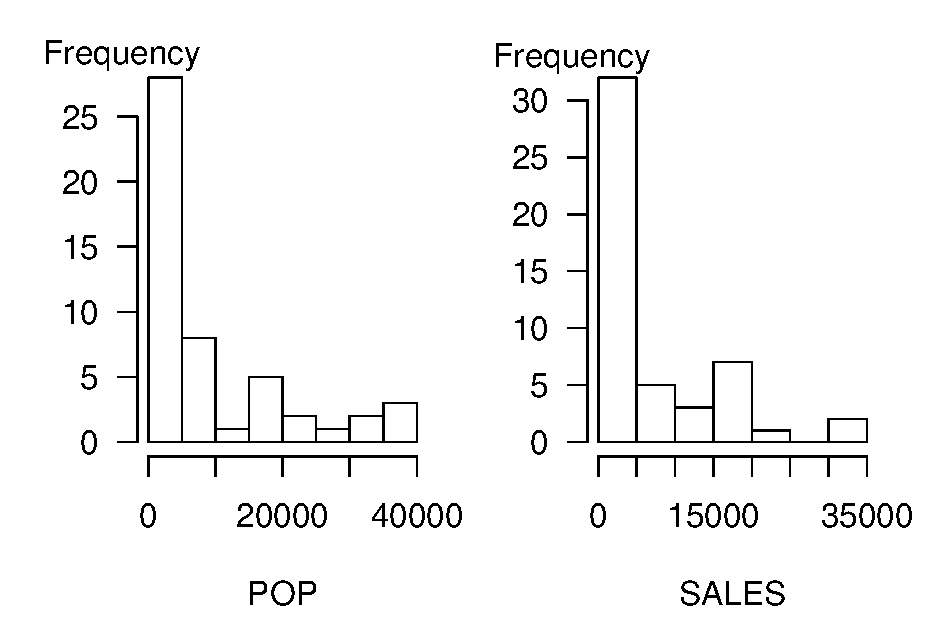
\includegraphics[width=0.6\textwidth]
    {Chapter2/F2HistPopSales.eps}
    \caption{\label{F2:HistPopSales} \small Histograms of Population and Sales.
    Each distribution is skewed to the right, indicating that there are many
    small areas compared to a few areas with larger sales and populations.}
  \end{center}
\end{figure}

\begin{table}[h] \scalefont{0.9}
\caption{\label{T2:SummaryStats}
Summary Statistics of Each Variable}
\begin{tabular}{lrrrrr}
\hline
&  &  & Standard &  &  \\
Variable & Mean & Median & Deviation & Minimum & Maximum \\ \hline
POP & 9,311 & 4,406 & 11,098 & 280 & 39,098 \\
SALES & 6,495 & 2,426 & 8,103 & 189 & 33,181 \\ \hline
\end{tabular}


\textit{Source: Frees and Miller (2003).}
 \scalefont{1.1111}
\end{table}

\bigskip

As Table \ref{T2:SummaryStats} shows, the basic summary statistics
give useful ideas of the structure of key features of the data.
After we understand the information in each variable in isolation of
the other, we can begin exploring the relationship between the two
variables.

\linetjed

\subsubsection*{Scatter Plot and Correlation Coefficients - Basic Summary
Tools}\index{plots!scatter}

The basic graphical tool used to investigate the relationship
between the two variables is a \emph{scatter plot} such as in Figure
\ref{F2:SalesVsPoP}. Although we may lose the exact values of the
observations when graphing data, we gain a visual impression of the
relationship between population and sales. From Figure
\ref{F2:SalesVsPoP} we see that areas with larger populations tend
to purchase more lottery tickets. How strong is this relationship?
Can knowledge of the area's population help us anticipate the
revenue from lottery sales? We explore these two questions below.

\begin{figure}[ht]
%\flushleft
    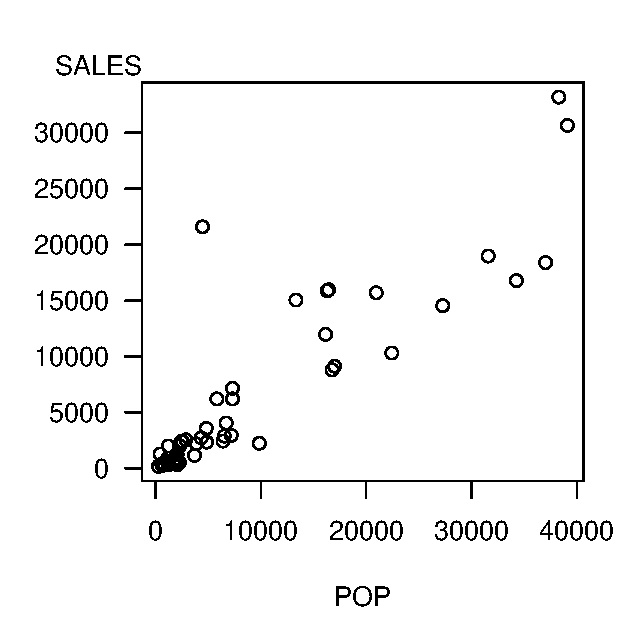
\includegraphics[width=0.6\textwidth]{Chapter2/F2SalesVsPoP.eps}
    \caption{\label{F2:SalesVsPoP} \small A scatter plot of the lottery data. Each of the 50
     plotting symbols corresponds to a zip code in the study. This figure suggests
     that postal areas with larger populations have larger lottery revenues.}
\end{figure}


One way to summarize the strength of the relationship between two
variables is through a \emph{correlation} statistic.

\bigskip

\boxedjed

\index{correlation coefficients!Pearson}\index{correlation
coefficients!ordinary}\index{symbols!$s_x$, sample standard
deviation of \{$x_1, \ldots, x_n$\}}\index{symbols!$s_y$, sample
standard deviation}

\textit{Definition}. The \emph{ordinary, or Pearson, correlation}
coefficient is defined as
\begin{equation*}
r=\frac{1}{(n-1)s_xs_y}\sum_{i=1}^{n}\left(
x_{i}-\overline{x}\right) \left( y_{i}-\overline{y}\right) .
\end{equation*}

\bigskip

\noindent Here, we use the sample standard deviation $s_y =
\sqrt{(n-1)^{-1} \sum_{i=1}^{n}\left( y_i -
\overline{y}\right)^{2}}$ defined in Section 1.2, with similar
notation for $s_x$.

\end{boxedminipage}

\bigskip

Although there are other correlation statistics, the correlation
coefficient devised by Pearson (1895) has several desirable
properties. One important property is that, for any data set, $r$ is
bounded by -1 and 1, that is, $-1\leq r\leq 1$. (Exercise 2A.9
provides steps for you to check this property.) If $r$ is greater
than zero, the variables are said to be \emph{(positively)
correlated}. If $r$ is less than zero, the variables are said to be
\emph{negatively correlated}. The larger the coefficient is in
absolute value, the stronger is the relationship. In fact, if $r=1$,
then the variables are perfectly correlated. In this case, all of
the data lie on a straight line that goes through the lower left and
upper right-hand quadrants. If $r=-1$, then all of the data lie on a
line that goes through the upper left and lower right-hand
quadrants. The coefficient $r$ is a measure of a \emph{linear}
relationship between two variables.

\marginparjed{The coefficient $r$ is a measure of a linear
relationship between two variables.}

The correlation coefficient is said to be \emph{location and scale
invariant}. Thus, each variable's center of location does not matter
in the calculation of $r$. For example, if we add \$100 to the sales
of each zip code, each $y_i$ will increase by 100. However,
$\overline{y}$, the average purchase price will also increase by 100
so that the deviation $y_i - \overline{y}$ remains unchanged, or
invariant. Further, the scale of each variable does not matter in
the calculation of $r$. For example, suppose we divide each
population by 1000 so that $x_i$ now represents population in
thousands. Thus, $\overline{x}$\ is also divided by 1000 and you
should check that $s_x$ is also divided by 1000. Thus, the
standardized version of $x_i$, $\left( x_i-\overline{x}\right)
/s_x$, remains unchanged, or invariant. Many statistical packages
compute a standardized version of a variable by subtracting the
average and dividing by the standard deviation. Now, let's use
$y_{i,std}=\left( y_i- \overline{y}\right) /s_y$ and
$x_{i,std}=\left( x_i-\overline{x} \right) /s_x$ to be the
standardized versions of $y_i$ and $x_i$, respectively. With this
notation, we can express the correlation coefficient as
$r=(n-1)^{-1}\sum_{i=1}^{n}x_{i,std}\times y_{i,std}.$

The correlation coefficient is said to be a \emph{dimensionless
measure}. This is because we have taken away dollars, and all other
units of measures, by considering the standardized variables
$x_{i,std}$ and $y_{i,std}$. Because the correlation coefficient
does not depend on units of measure, it is a statistic that can
readily be compared across different data sets.

\marginparjed{The correlation coefficient is location and scale
invariant. It is dimensionless.}

\index{explanatory variable!quadratic}

In the world of business, the term ``correlation'' is often used as
synonymous with the term ``relationship.'' For the purposes of this
text, we use the term correlation when referring only to linear
relationships. The classic nonlinear relationship is $y=x^{2}$, a
quadratic relationship. Consider this relationship and the
fictitious data set for $x$, $\{-2,1,0,1,2\}$. Now, as an exercise
(2.\ref{Ex:ZeroCorr}), produce a rough graph of the data set:

\scalefont{0.9}
\begin{center}
$
\begin{tabular}{l|rrrrr}
\hline
$i$ & 1 & 2 & 3 & 4 & 5 \\
$x_i$ & -2 & -1 & 0 & 1 & 2 \\
$y_i$ & 4 & 1 & 0 & 1 & 4 \\ \hline
\end{tabular}
$
\end{center}
\scalefont{1.1111}

\noindent The correlation coefficient for this data set turns out to be $r=0$
(check this). Thus, despite the fact that there is a perfect relationship
between $x$ and $y$ ($=x^{2}$), there is a zero correlation. Recall that
location and scale changes are not relevant in correlation discussions, so
we could easily change the values of $x$ and $y$ to be more representative
of a business data set.

How strong is the relationship between $y$ and $x$ for the lottery
data? Graphically, the response is a scatter plot, as in Figure
\ref{F2:SalesVsPoP}. Numerically, the main response is the
correlation coefficient which turns out to be $r$ = 0.886 for this
data set. We interpret this statistic by saying that SALES and POP
are (positively) correlated. The strength of the relationship is
strong because $r$ = 0.886 is close to one. In summary, we may
describe this relationship by saying that there is a strong
correlation between SALES and POP.

\subsubsection*{Method of Least Squares}\index{least squares!method}

Now we begin to explore the question, ``Can knowledge of population
help us understand sales?'' To respond to this question, we identify
sales as the \emph{response}, or \emph{dependent, variable}. The
population variable, which is used to help understand sales, is
called the \emph{explanatory}, or \emph{independent, variable}.

Suppose that we have available the sample data of fifty sales $\{y_1, \ldots, y_{50} \}$ and your job
is to predict the sales of a randomly selected ZIP code. Without
knowledge of the population variable, a sensible predictor is simply
$\overline{y}=6,495$, the average of the available sample.
Naturally, you anticipate that areas with larger populations will
have larger sales. That is, if you also have knowledge of
population, then can this estimate be improved? If so, then by how
much?

To answer these questions, the first step assumes an approximate
linear relationship between $x$ and $y$. To fit a line to our data
set, we use the \emph{method of least squares}. We need a general
technique so that, if different analysts agree on the data and agree
on the fitting technique, then they will agree on the line. If
different analysts fit a data set using eyeball approximations, in
general they will arrive at different lines, even using the same
data set.

The method\ begins with the line $y=b_0^{\ast}+b_1^{\ast}x$, where
the intercept and slope, $b_0^{\ast}$ and $b_1^{\ast}$, are merely
generic values. For the $i$th observation, $y_i-\left(
b_0^{\ast}+b_1^{\ast}x_i\right) $ represents the deviation of the
observed value $y_i$ from the line at $x_i$. The quantity
\begin{equation*}
SS(b_0^{\ast},b_1^{\ast})=\sum_{i=1}^{n}\left( y_i-\left(
b_0^{\ast}+b_1^{\ast}x_i\right) \right) ^{2}
\end{equation*}
represents the sum of squared deviations for this candidate line.
The least squares method consists of determining the values of
$b_0^{\ast}$ and $b_1^{\ast}$\ that minimize
$SS(b_0^{\ast},b_1^{\ast})$. This is an easy problem that can be
solved by calculus, as follows. Taking partial derivatives with
respect to each argument yields
\begin{equation*}
\frac{\partial }{\partial
b_0^{\ast}}SS(b_0^{\ast},b_1^{\ast})=\sum_{i=1}^{n}(-2)\left(
y_i-\left( b_0^{\ast}+b_1^{\ast}x_i\right) \right)
\end{equation*}
and
\begin{equation*}
\frac{\partial }{\partial
b_1^{\ast}}SS(b_0^{\ast},b_1^{\ast})=\sum_{i=1}^{n}(-2x_i)\left(
y_i-\left( b_0^{\ast}+b_1^{\ast}x_i\right) \right) .
\end{equation*}
The reader is invited to take second partial derivatives to ensure
that we are minimizing, not maximizing, this function. Setting these
quantities equal to zero \ and canceling constant terms yields
\begin{equation*}
\sum_{i=1}^{n}\left( y_i-\left( b_0^{\ast}+b_1^{\ast}x_i\right)
\right) =0
\end{equation*}
and
\begin{equation*}
\sum_{i=1}^{n}x_i\left( y_i-\left( b_0^{\ast}+b_1^{\ast}x_i\right)
\right) =0,
\end{equation*}
which are known as the \emph{normal equations}. Solving these
equations yields the values of $b_0^{\ast}$ and $b_1^{\ast}$ that
minimize the sum of squares, as follows.\index{normal equations}

\bigskip

\boxedjed \index{least squares!intercept}\index{least
squares!slope}\index{symbols!$b_0$, least squares
intercept}\index{symbols!$b_1$, least squares
slope}\index{symbols!$\widehat{y}$, fitted value of $y$}

\textit{Definition. }The \emph{least squares intercept and slope
estimates} are

\begin{equation*}
b_1=r\frac{s_y}{s_x}~~~~~\mathrm{and}~~~~~b_0=\overline{y}-b_1
\overline{x}.
\end{equation*}
The line that they determine, $\widehat{y}=b_0+b_1x$, is called the
\emph{fitted regression line}.

\end{boxedminipage}
\bigskip

\noindent We have dropped the asterisk, or star, notation because
$b_0$ and $b_1$ are no longer ``candidate'' values.

Does this procedure yield a sensible line for our Wisconsin lottery
sales? Earlier, we computed $r=0.886$. From this and the basic
summary statistics in Table \ref{T2:SummaryStats}, we have $b_1 =
0.886 \left( 8,103\right) /11,098=0.647$ and $b_0 =
6,495-(0.647)9,311 = 469.7.$ This yields the fitted regression line
\begin{equation*}
\widehat{y} = 469.7 + (0.647)x.
\end{equation*}
The carat, or ``hat,'' on top of the $y$ reminds us that this
$\widehat{y}$, or $\widehat{SALES}$, is a fitted value. One
application of the regression line is to estimate sales for a
specific population say, $x=10,000$. The estimate is the height of
the regression line, which is $469.7 + (0.647)(10,000) = 6,939.7$.

\linejed

\index{examples!summarizing simulations}\index{actuarial \&
financial terms and concepts!value-at-risk, VaR}\index{actuarial \&
financial terms and concepts!conditional tail expectation, CTE}

\textbf{Example: Summarizing Simulations.}\ecaptionjed{Summarizing
Simulations} Regression analysis is a tool for summarizing complex
data. In practical work, actuaries often simulate complicated
financial scenarios; it is often overlooked that regression can be
used to summarize relationships of interest.

To illustrate, Manistre and Hancock (2005) simulated many
realizations of a 10-year European put option and demonstrated the
relationship between two actuarial risk measures, the value-at-risk
(VaR) and the conditional tail expectation (CTE). For one example,
these authors examined lognormally distributed stock returns with an
initial stock price of \$100, so that in 10 years the price of the
stock would be distributed as
\begin{equation*}
S(Z)=100 \exp \left( (.08) 10 + .15 \sqrt{10} Z \right),
\end{equation*}
based on an annual mean return of 10\%, standard deviation 15\% and
the outcome from a standard normal random variable $Z$. The put
option pays the difference between the strike price, that will be
taken to be 110 for this example, and $S(Z)$. The present value of
this option is
\begin{equation*}
C(Z)= \mathrm{e}^{-0.06(10)} \mathrm{max} \left(0, 110-S(Z) \right),
\end{equation*}
based on a 6\% discount rate.

To estimate the VaR and CTE, for each $i$, 1000 i.i.d. standard
normal random variables were simulated and used to calculate 1000
present values, $C_{i1}, \ldots, C_{i,1000}.$ The 95th percentile of
these present values is the estimate of the value at risk, denoted
as $VaR_i.$ The average of the highest 50 ($= (1-.05) \times 1000$)
of the present values is the estimate of the conditional tail
expectation, denoted as $CTE_i$. Manistre and Hancock (2005)
performed this calculation $i=1, \ldots, 1000$ times; the result is
presented in Figure \ref{F2:VarCTE}. The scatterplot shows a strong
but not perfect relationship between the $VaR$ and the $CTE$, the
correlation coefficient turns out to be $r=0.782$.


\begin{figure}[htp]
  \begin{center}
   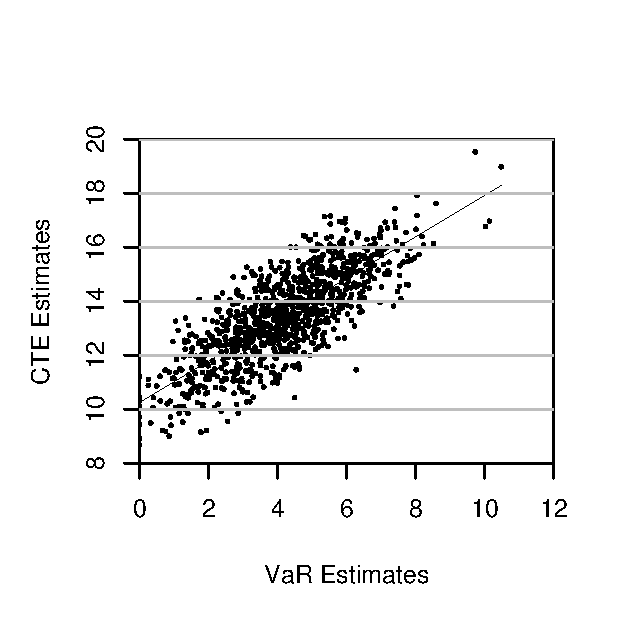
\includegraphics[width=0.6\textwidth]{Chapter2/VarCTEFig.eps}
    \caption{\label{F2:VarCTE} \small Plot of Conditional Tail Expectation (CTE) versus Value at Risk (VaR).
    Based on $n=1,000$ simulations from a 10-year European put bond. \textit{Source: Manistre and
Hancock (2005)}}
  \end{center}
\end{figure}

\linejed


\section{Basic Linear Regression Model}\index{regression model!basic linear}\index{regression model!simple linear}

The scatter plot, correlation coefficient and the fitted regression
line are useful devices for summarizing the relationship between two
variables for a specific data set. To infer general relationships,
we need models to represent outcomes of broad populations.

This chapter focuses on a ``basic linear regression'' model. The
``linear regression'' part comes from the fact that we fit a line to
the data. The ``basic'' part is because we use only one explanatory
variable, $x$. This model is also known as a ``simple'' linear
regression. This text avoids this language because it gives the
false impression that regression ideas and interpretations with one
explanatory variable are always straightforward.

We now introduce two sets of assumptions of the basic model, the
``observables'' and the ``error'' representations. They are
equivalent but each will help us as we later extend regression
models beyond the basics.\index{model assumptions!observables
representation}\index{symbols!$\beta_0$, (population) regression
intercept}\index{symbols!$\beta_1$, (population) regression
coefficient associated with $x_1$}

\begin{center}\scalefont{0.9}
\begin{tabular}{c}
\hline
Basic Linear Regression Model \\
Observables Representation Sampling Assumptions \\ \hline
\multicolumn{1}{l}{F1. $\mathrm{E}~y_i=\beta_0 + \beta_1 x_i $.} \\
\multicolumn{1}{l}{F2. $\{x_1,\ldots ,x_n\}$ are non-stochastic
variables.} \\
\multicolumn{1}{l}{F3. $\mathrm{Var}~y_i=\sigma ^{2}$.} \\
\multicolumn{1}{l}{F4. \{$y_i$\} are independent random variables.} \\
\hline
\end{tabular}\scalefont{1.1111}
\end{center}

The ``observables representation'' focuses on variables that we can
see (or observe), $(x_i,y_i)$. Inference about the distribution of
$y$ is conditional on the observed explanatory variables, so that we
may treat $\{x_1,\ldots ,x_n\}$ as non-stochastic variables
(assumption F2). When considering types of sampling mechanisms for
$(x_i,y_i)$, it is convenient to think of a \emph{stratified random
sampling} scheme, where values of $\{x_1,\ldots ,x_n\}$ are treated
as the strata, or group. Under stratified sampling, for each unique
value of $x_i$, we draw a random sample from a population. To
illustrate, suppose you are drawing from a database of firms to
understand stock return performance ($y$) and wish to stratify based
on the size of the firm. If the amount of assets is a
continuous variable, then we can imagine drawing a sample of size 1
for each firm. In this way, we hypothesize a distribution of stock
returns conditional on firm asset size.

\emph{Digression}: You will often see reports that summarize results for the ``top 50
managers'' or the ``best 100 universities,'' measured by some
outcome variable. In regression applications, make sure that you do
not select observations based on a dependent variable, such as
the highest stock return, because this is stratifying
based on the $y$, not the $x$. Chapter 6 will discuss sampling procedures in greater detail.

Stratified sampling also provides motivation for assumption F4, the
independence among responses. One can motivate assumption F1 by
thinking of $(x_i,y_i)$ as a draw from a population, where the mean
of the conditional distribution of $y_i$ given \{$x_i$\} is linear
in the explanatory variable. Assumption F3 is known as
\emph{homoscedasticity} that we will discuss extensively in Section
5.7. See Goldberger (1991) for additional background on this
representation.\index{homoscedasticity}

A fifth assumption that is often implicitly used is:

\begin{center}
F5. \{$y_i$\} are normally distributed.
\end{center}

\noindent This assumption is not required for many statistical inference
procedures because central limit theorems provide approximate normality for
many statistics of interest. However, formal justification for some, such as
$t$-statistics, do require this additional assumption.

In contrast to the observables representation, an alternative set of
assumptions focuses on the deviations, or ``errors,'' in the
regression, defined as $\varepsilon_i=y_i-\left( \beta_0 + \beta_1
x_i \right) $.\index{model assumptions!error
representation}\index{symbols!$\varepsilon_i$, ``error,'' or
disturbance term}

\begin{center}\scalefont{0.9}
\begin{tabular}{c}
\hline
Basic Linear Regression Model \\
Error Representation Sampling Assumptions \\ \hline
\multicolumn{1}{l}{E1. $y_i=\beta_0+\beta_1 x_i + \varepsilon _i$.}
\\
\multicolumn{1}{l}{E2. $\{x_1,\ldots ,x_n\}$ are non-stochastic
variables.} \\
\multicolumn{1}{l}{E3. $\mathrm{E}~\varepsilon _i=0$ and $\mathrm{Var}~\varepsilon _i=\sigma ^{2}$.} \\
\multicolumn{1}{l}{E4. \{$\varepsilon _i$\} are independent random
variables.} \\ \hline
\end{tabular}\scalefont{1.1111}
\end{center}

The ``error representation'' is based on the Gaussian theory of
errors (see Stigler, 1986, for a historical background). Assumption
E1 assumes that $y$ is in part due to a linear function of the
observed explanatory variable, $x$. Other unobserved variables that
influence the measurement of $y$ are interpreted to be included in
the ``error'' term $\varepsilon _i$, which is also known as the
``disturbance'' term. The independence of errors, E4, can be
motivated by assuming that \{$\varepsilon _i$\} are realized through
a simple random sample from an unknown population of errors.

Assumptions E1-E4 are equivalent to F1-F4. The error representation
provides a useful springboard for motivating goodness of fit
measures (Section \ref{S2:SummStats}). However, a drawback of the
error representation is that it draws the attention from the
observable quantities $(x_i,y_i)$ to an unobservable quantity,
\{$\varepsilon _i$\}. To illustrate, the sampling basis, viewing
\{$\varepsilon _i$\} as a simple random sample, is not directly
verifiable because one cannot directly observe the sample \{$
\varepsilon _i$\}. Moreover, the assumption of additive errors in E1
will be troublesome when we consider nonlinear regression models.

Figure \ref{F2:NormalCurve} illustrates some of the assumptions of
the basic linear regression model. The data ($x_1,y_1$), ($x_2,y_2$)
and ($x_3,y_3$) are observed and are represented by the circular
opaque plotting symbols. According to the model, these observations
should be close to the regression line $\mathrm{E}~y = \beta_0 +
\beta_1 x$. Each deviation from the line is random. We will often
assume that the distribution of deviations may be represented by a
normal curve, as in Figure \ref{F2:NormalCurve}.


\begin{figure}[htp]
  \begin{center}
    %  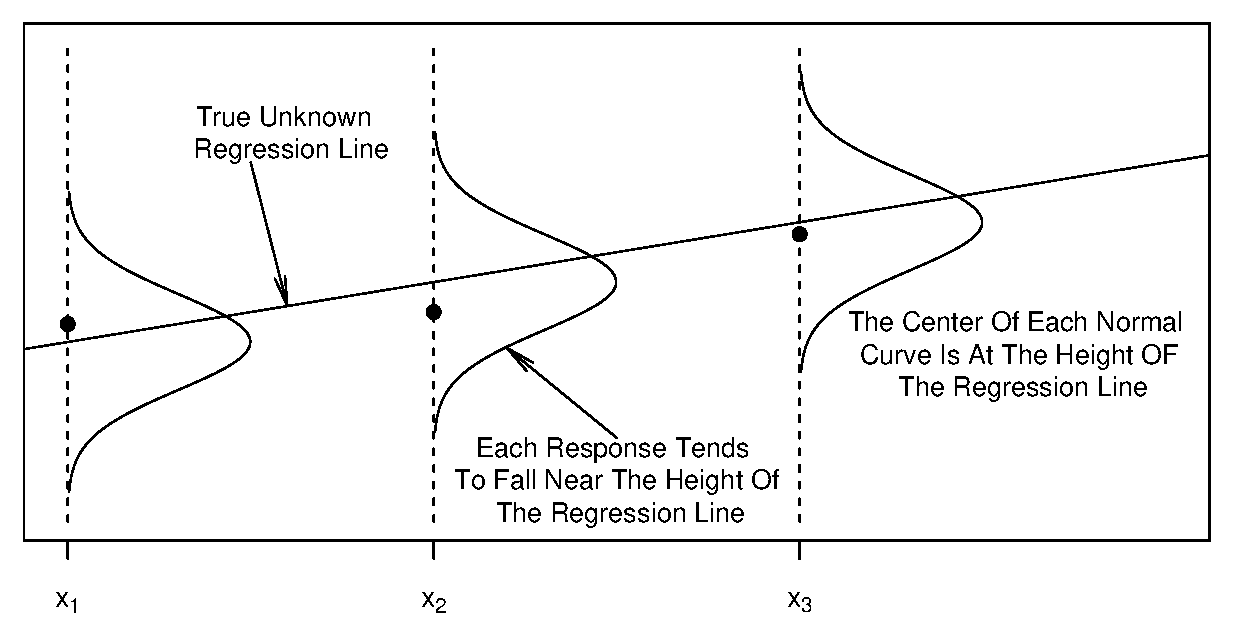
\includegraphics[width=1\textwidth,angle=270,scale=.75]{Chapter2/F2NormalCurve.ps}
    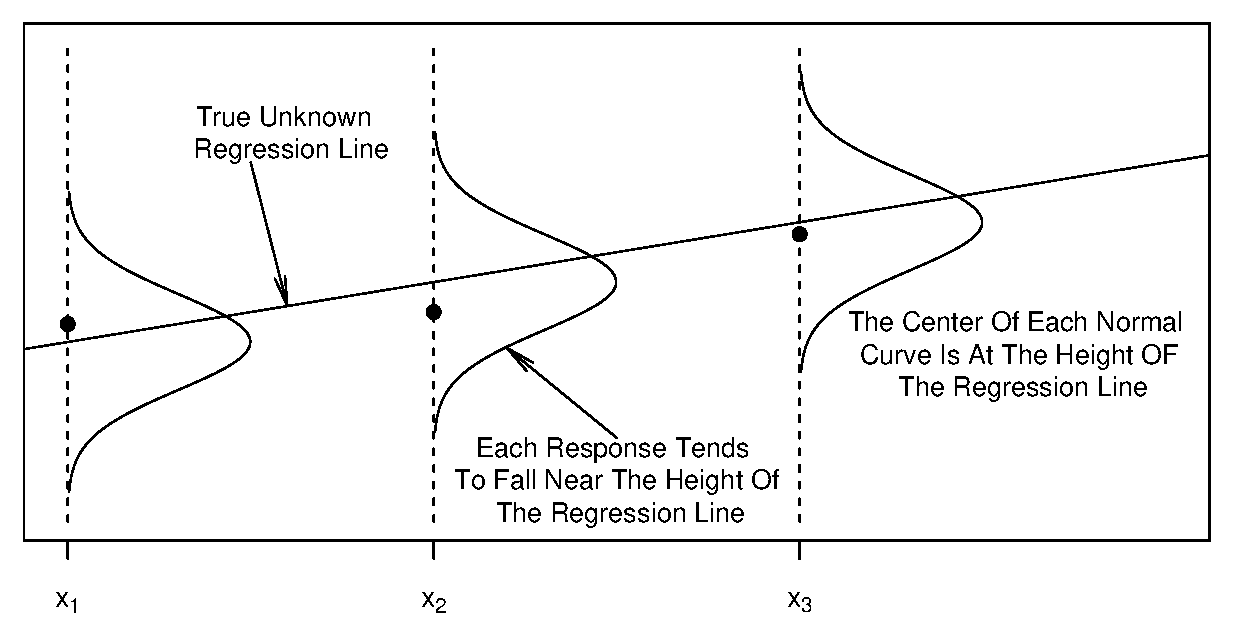
\includegraphics[width=0.8\textwidth]{Chapter2/F2NormalCurve.eps}
    \caption{\label{F2:NormalCurve} \small The distribution of the response varies by the level of the
explanatory variable.}
  \end{center}
\end{figure}

The basic linear regression model assumptions describe the
underlying population. Table \ref{T2:SumPopSample} highlights the
idea that characteristics of this population can be summarized by
the parameters $\beta_0$, $\beta_1$ and $\sigma ^{2}$. In Section
2.1, we summarized data from a sample, introducing the statistics
$b_0$ and $b_1$. Section \ref{S2:SummStats} will introduce $s^{2}$,
the statistic corresponding to the parameter $\sigma ^{2}$.

\begin{table}[h]
\caption{\label{T2:SumPopSample} Summary Measures of the Population
and Sample}
\begin{tabular}{ccccc}
\hline
Data & Summary & \multicolumn{2}{c}{Regression} & Variance \\
& Measures & \multicolumn{2}{c}{Line} &  \\ \cline{3-4}
\vspace{-0.1in} \\& & Intercept & Slope &  \\ \hline
Population & Parameters & $\beta_0$ & $\beta_1$ & $\sigma ^{2}$ \\
Sample & Statistics & $b_0$ & $b_1$ & $s^2$ \\ \hline
\end{tabular}
\end{table}

\section{Is the Model Useful? Some Basic Summary
Measures}\label{S2:SummStats}

Although statistics is the science of summarizing data, it is also
the art of arguing with data. This section develops some of the
basic tools used to justify the basic linear regression model. A
scatter plot may provide strong \emph{visual} evidence that $x$
influences $y$; developing \emph{numerical} evidence will enable us
to quantify the strength of the relationship. Further, numerical
evidence will be useful when we consider other data sets where the
graphical evidence is not compelling.

\subsection{Partitioning the Variability}

The squared deviations, $\left( y_i-\overline{y}\right) ^2$, provide
a basis for measuring the spread of the data. If we wish to estimate
the $i$th dependent variable \emph{without} knowledge of $x$, then
$\overline{y}$\ is an appropriate estimate and $y_i- \overline{y}$
represents the deviation of the estimate. We use
$Total~SS=\sum_{i=1}^{n}\left( y_i-\overline{y}\right) ^2$, the
total sum of squares, to represent the variation in all of the
responses.\index{symbols!$Total~SS$, total sum of squares}

Suppose now that we also have knowledge of $x$, an explanatory
variable. Using the fitted regression line, for each observation we
can compute the corresponding\emph{\ fitted value}, $\widehat{y}_i =
b_0 + b_1x_i$. The fitted value is our estimate \emph{with}
knowledge of the explanatory variable. As before, the difference
between the response and the fitted value, $y_i- \widehat{y}_i$,
represents the deviation of this estimate. We now have two
``estimates'' of $y_i$, these are $\widehat{y}_i$ and
$\overline{y}$. Presumably, if the regression line is useful, then $
\widehat{y}_i$ is a more accurate measure than $\overline{y}$. To
judge this usefulness, we algebraically decompose the total
deviation as:
\begin{equation}\label{E2:deviationdecomp}
\begin{tabular}{ccccc}
$\underbrace{y_i-\overline{y}}$ & = &
$\underbrace{y_i-\widehat{y}_i}$
& + & $\underbrace{\widehat{y}_i-\overline{y}}$ \\
{\small total} & {\small =} & {\small unexplained} & {\small +} &
{\small
explained} \\
{\small deviation} &  & {\small deviation} &  & {\small deviation}
\end{tabular}
\end{equation}
Interpret this equation as ``the deviation without knowledge of $x$
equals the deviation with knowledge of $x$ plus the deviation
explained by $x$.'' Figure \ref{F2:ANOVADecomp} is a geometric
display of this decomposition. In the figure, an observation above
the line was chosen, yielding a positive deviation from the fitted
regression line, to make the graph easier to read. A good exercise
is to draw a rough sketch corresponding to Figure
\ref{F2:ANOVADecomp} with an observation below the fitted regression
line.

\begin{figure}[htp]
  \begin{center}
    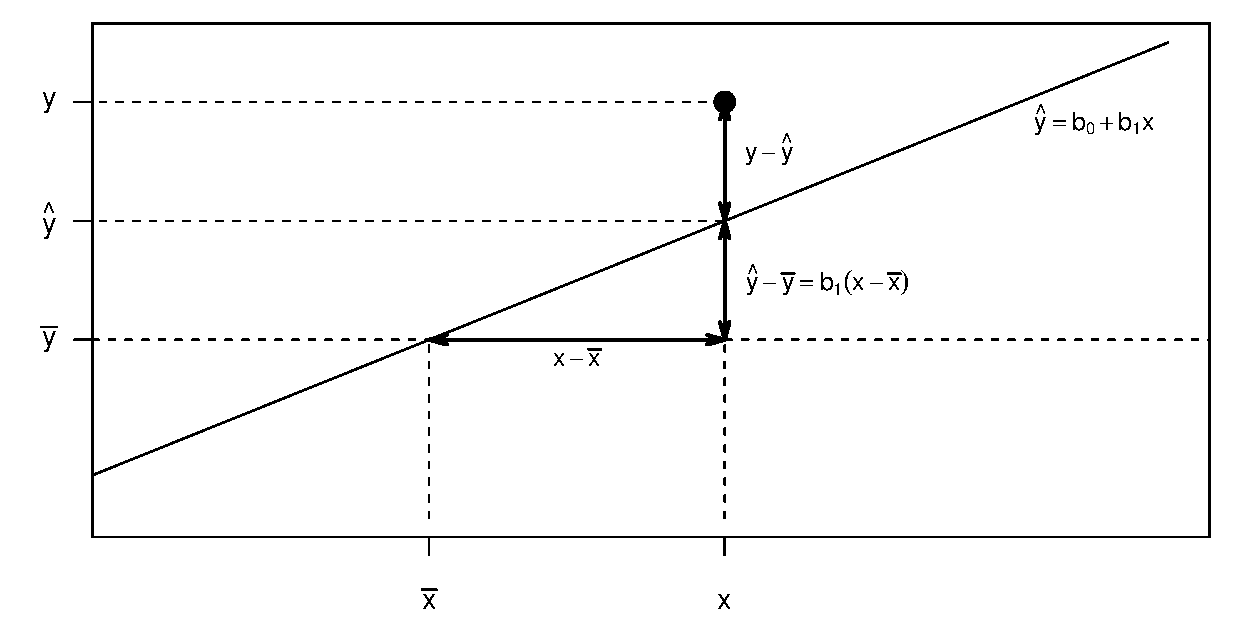
\includegraphics[width=0.8\textwidth]{Chapter2/F2ANOVADecomp.eps}
    \caption{\label{F2:ANOVADecomp} \small Geometric display of the deviation decomposition.}
  \end{center}
\end{figure}

\bigskip

Now, from the algebraic decomposition in equation
(\ref{E2:deviationdecomp}), square each side of the equation and sum
over all observations. After a little algebraic manipulation, this
yields
\begin{equation}\label{E2:ANOVADecomposition}
\sum_{i=1}^{n}\left( y_i-\overline{y}\right) ^2=\sum_{i=1}^{n}\left(
y_i-\widehat{y}_i\right) ^2+\sum_{i=1}^{n}\left( \widehat{y}_i-
\overline{y}\right) ^2.
\end{equation}
We rewrite this as $Total~SS=Error~SS+Regression~SS$ where $SS$ stands for
sum of squares. We interpret:

\begin{itemize}
\item $Total~SS$ as the total variation without knowledge of $x$,

\item $Error~SS$ as the total variation remaining after the introduction of $x$, and

\item $Regression~SS$ as the difference between the $Total~SS$ and $Error~SS$
, or the total variation ``explained'' through knowledge of $x$.
\end{itemize}

\index{symbols!$Error~SS$, error sum of
squares}\index{symbols!$Regression~SS$, regression sum of squares}



\noindent When squaring the right-hand side of equation
(\ref{E2:deviationdecomp}), we have the cross-product term $2\left(
y_i-\widehat{y}_i\right) \left( \widehat{y}_i-\overline{y}\right) $.
With the ``algebraic manipulation,'' one can check that the sum of
the cross-products over all observations is zero. This result is not
true for all fitted lines but is a special property of the least
squares fitted line.

In many instances, the variability decomposition is reported through only a
single statistic.

\bigskip\index{goodness of fit statistics!coefficient of
determination, $R^2$}\index{symbols!$R^2$, coefficient of
determination}

\boxedjed

\textit{Definition.} The \emph{coefficient of determination} is
denoted by the symbol $R^2$, called ``$R$-square,'' and defined as
\begin{equation*}
R^2=\frac{Regression~SS}{Total~SS}.
\end{equation*}

\end{boxedminipage}
\bigskip

\noindent We interpret $R^2$ to be the proportion of variability
explained by the regression line. In one extreme case where the
regression line fits the data perfectly, we have $Error~SS=0$ and
$R^2=1$. In the other extreme case where the regression line
provides no information about the response, we have
$Regression~SS=0$ and $R^2=0.$ The coefficient of determination is
constrained by the inequalities $0 \leq R^2 \leq 1$ with larger
values implying a better fit.

\subsection{The Size of a Typical Deviation: \textit{s}}

In the basic linear regression model, the deviation of the response
from the regression line, $y_i-\left( \beta_0+\beta_1x_i\right) $,
is not an observable quantity because the parameters $\beta_0$ and
$\beta_1$ \ are not observed. However, by using estimators $b_0$ and
$b_1$, we can approximate this deviation using
\begin{equation*}
e_i=y_i-\widehat{y}_i=y_i-\left( b_0+b_1x_i\right) ,
\end{equation*}
known as the \emph{residual}.\index{residual}\index{symbols!$e_i$,
residual}

Residuals will be critical to developing strategies for improving
model specification in Section \ref{S2:ResidualAnalsis}. We now show
how to use the residuals to estimate $\sigma ^2$. From a first
course in statistics, we know that if one could observe the
deviations $\varepsilon _i$, then a desirable estimate of $\sigma
^2$\ would be $(n-1)^{-1}\sum_{i=1}^{n}\left( \varepsilon
_i-\overline{\varepsilon }\right) ^2$. Because \{$\varepsilon _i$\}
are not observed, we use the following.

\bigskip\index{symbols!$s^2$, mean square error}
\index{symbols!$s$, residual standard deviation}

\boxedjed

\textit{Definition}. An estimator of $\sigma ^2$, the \emph{mean
square error (MSE)}, is defined as
\begin{equation}
s^2=\frac{1}{n-2}\sum_{i=1}^{n}e_i{}^2.  \label{BLRs2}
\end{equation}
The positive square root, $s=\sqrt{s^2},$ is called the
\emph{residual standard deviation}.

\end{boxedminipage}
\bigskip

Comparing the definitions of $s^2$ and
$(n-1)^{-1}\sum_{i=1}^{n}\left( \varepsilon _i-\overline{\varepsilon
}\right) ^2$, you will see two important differences. First, in
defining $s^2$ we have not subtracted the average residual from each
residual before squaring. This is because the average residual is
zero, a special property of least squares estimation (see Exercise
2.\ref{Ex:AverageResid}). This result can be shown using algebra and
is guaranteed for all data sets.

\marginparjed{$s^2$ is an unbiased estimator of $\sigma ^2$.}

Second, in defining $s^2$ we have divided by $n-2$ instead of $n-1$.
Intuitively, dividing by either $n$ or $n-1$ tends to underestimate
$\sigma ^2$. The reason is that, when fitting lines to data, we need
at least two observations to determine a line. For example, we must
have at least three observations for there to be any variability
about a line. How much ``freedom'' is there for variability about a
line? We will say that the error degrees of freedom is the number of
observations available, $n$, minus the number of observations needed
to determine a line, 2 (with symbols, $df=n-2$). However, as we saw
in the least squares estimation subsection, we do not need to identify
two actual observations to determine a line. The idea is that if an
analyst knows the line and $n-2$ observations, then the remaining
two observations can be determined, without variability. When
dividing by $n-2$, it can be shown that $s^2$ is an unbiased
estimator of $\sigma ^2$.

We can also express $s^2$ in terms of the sum of squares quantities.
That is,

\begin{equation*}
s^2=\frac{1}{n-2}\sum_{i=1}^{n}\left( y_i-\widehat{y}_i\right) ^2=
\frac{Error~SS}{n-2}=MSE.
\end{equation*}

\index{analysis of variance, ANOVA, table}

This leads us to the \emph{analysis of variance}, or \emph{ANOVA},
table:

\scalefont{0.8}

\begin{center}
\begin{tabular}{llcl}
\hline
\multicolumn{4}{c}{ANOVA\ Table} \\ \hline
Source & Sum of Squares & $df$ & Mean Square \\ \hline
Regression & $Regression~SS$ & $1$ & $Regression~MS$ \\
Error & $Error~SS$ & $n-2$ & $MSE$ \\
Total & $Total~SS$ & $n-1$ &  \\ \hline
\end{tabular}
\end{center}

\scalefont{1.25}

\noindent The ANOVA table is merely a bookkeeping device used to
keep track of the sources of variability; it routinely appears in
statistical software packages as part of the regression output. The
mean square column figures are defined to be the sums of square
($SS$) figures divided by their respective degrees of freedom
($df$). In particular, the mean square for errors ($MSE$) equals $
s^2$ and the regression sum of squares equals the regression mean
square. This latter property is specific to the regression with one
variable case; it is not true where we consider more than one
explanatory variable.

The error degrees of freedom in the ANOVA table is $n-2$. The total degrees
of freedom is $n-1$, reflecting the fact that the total sum of squares is centered about the mean (at least two observations are required for positive variability). The single degree of freedom associated with the regression
portion means that the slope, plus one observation, is enough information to
determine the line. This is because it takes two observations to determine a
line and at least three observations for there to be any variability about
the line.

The analysis of variance table for the lottery data is:

\scalefont{0.8}

\begin{center}
\begin{tabular}{llll}
\hline
\multicolumn{4}{c}{ANOVA\ Table} \\ \hline
Source & Sum of Squares & $df$ & Mean Square \\ \hline
Regression & \multicolumn{1}{r}{2,527,165,015} & \multicolumn{1}{r}{1} &
\multicolumn{1}{r}{2,527,165,015} \\
Error & \multicolumn{1}{r}{690,116,755} & \multicolumn{1}{r}{48} &
\multicolumn{1}{r}{14,377,432} \\
Total & \multicolumn{1}{r}{3,217,281,770} & \multicolumn{1}{r}{49} &
\multicolumn{1}{r}{} \\ \hline
\end{tabular}
\end{center}
\scalefont{1.25}

 \noindent From this table, you can check that
$R^2=78.5\%$ and $s=3,792.$

\section{Properties of Regression Coefficient Estimators}

The least squares estimates can be expressed as weighted sum of the
responses. To see this, define the weights
\begin{equation*}
w_i=\frac{x_i-\overline{x}}{s_x^2(n-1)}.
\end{equation*}
Because the sum of $x$-deviations ($x_i-\overline{x}$) is zero, we
see that $\sum_{i=1}^{n}w_i=0$. Thus, we can express the slope
estimate
\begin{equation}
b_1=r\frac{s_y}{s_x}=\frac{1}{(n-1)s_x^2}\sum_{i=1}^{n}\left(
x_i-\overline{x}\right) \left( y_i-\overline{y}\right)
=\sum_{i=1}^{n}w_i\left( y_i-\overline{y}\right)
=\sum_{i=1}^{n}w_iy_i.  \label{weightb1}
\end{equation}

\noindent The exercises ask the reader to verify that $b_0$ can also
be expressed as a weighted sum of responses, so our discussion
pertains to both regression coefficients. Because regression
coefficients are weighted sums of responses, they can be affected
dramatically by unusual observations (see Section
\ref{S2:ResidualAnalsis}).

\marginparjed{Regression coefficients are weighted sums of the
responses.}

Because $b_1$ is a weighted sum, it is straightforward to derive the
expectation and variance of this statistic. By the linearity of
expectations and Assumption F1, we have
\begin{equation*}
\mathrm{E}~b_1=\sum_{i=1}^{n}w_i~\mathrm{E}~y_i=\beta_0\sum_{i=1}^{n}w_i+\beta_1\sum_{i=1}^{n}w_ix_i=\beta_1.
\end{equation*}
That is, $b_1$ is an unbiased estimator of $\beta_1$. Here, the sum
$ \sum_{i=1}^{n}w_ix_i$ $=$ \linebreak $\left[ s_x^2(n-1)\right]
^{-1}\sum_{i=1}^{n}\left( x_i-\overline{x}\right) x_i$ $=\left[
s_x^2(n-1)\right] ^{-1}\sum_{i=1}^{n}\left( x_i-\overline{x}\right)
^2=1.$ From the definition of the weights, some easy algebra also
shows that $\sum_{i=1}^{n}w_i^2=1/\left( s_x^2(n-1)\right) $.
Further, the independence of the responses implies that the variance
of the sum is the sum of the variances, and thus we have
\begin{equation*}
\mathrm{Var}~b_1=\sum_{i=1}^{n}w_i^2\mathrm{Var}~y_i=\frac{\sigma
^2}{s_x^2(n-1)}.
\end{equation*}
Replacing $\sigma ^2$\ by its estimator $s^2$ and taking square
roots leads to the following.

\bigskip\index{symbols!$se(b)$, standard error of $b$}

\boxedjed

\textit{Definition}. The \emph{standard error} of $b_1$, the
estimated standard deviation of $b_1$, is defined as
\begin{equation}
se(b_1)=\frac{s}{s_x\sqrt{n-1}}.  \label{seb1a}
\end{equation}

\end{boxedminipage}
\bigskip

This is our measure of the reliability, or precision, of the slope
estimator. Using equation (\ref{seb1a}), we see that $se(b_1)$ is
determined by three quantities, $n$, $s$ and $s_x$, as follows:

\marginparjed{A standard error is an estimated standard deviation.}


\begin{itemize}
\item If we have more observations so that $n$ becomes larger, then $
se(b_1)$ becomes smaller, other things equal.

\item If the observations have a greater tendency to lie closer to the line
so that $s$ becomes smaller, then $se(b_1)$ becomes smaller, other
things equal.

\item If values of the explanatory variable become more spread out so that $
s_x$ increases, then $se(b_1)$ becomes smaller, other things equal.
\end{itemize}

Smaller values of $se(b_1)$ offer a better opportunity to detect
relations between $y$ and $x$. Figure \ref{F2:BasicLSRE} illustrates
these relationships. Here, the scatter plot in the middle has the
smallest value of $se(b_1)$. Compared with the middle plot, the
left-hand plot has a larger value of $s$ and thus $se(b_1)$.
Compared with the right-hand plot, the middle plot has a larger
$s_x$, and thus smaller value of $se(b_1)$.

\noindent

\begin{figure}[htp]
  \begin{center}
    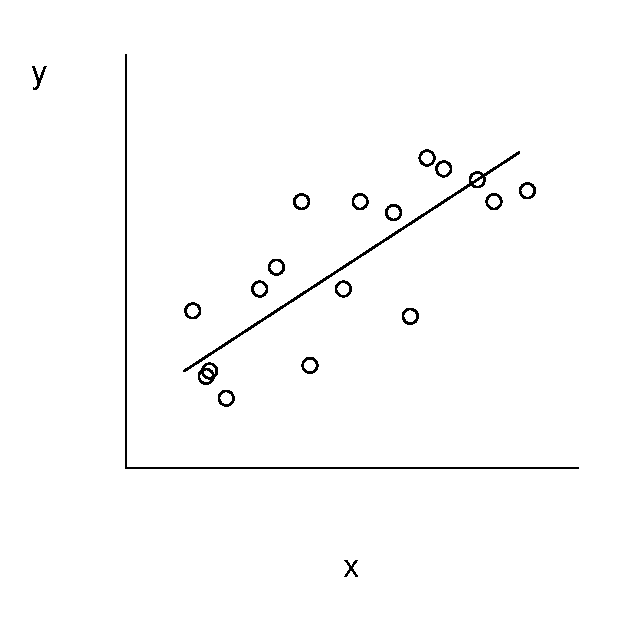
\includegraphics[height=1.8in,width=1.8in]{Chapter2/F2BasicLSRE1.eps}
    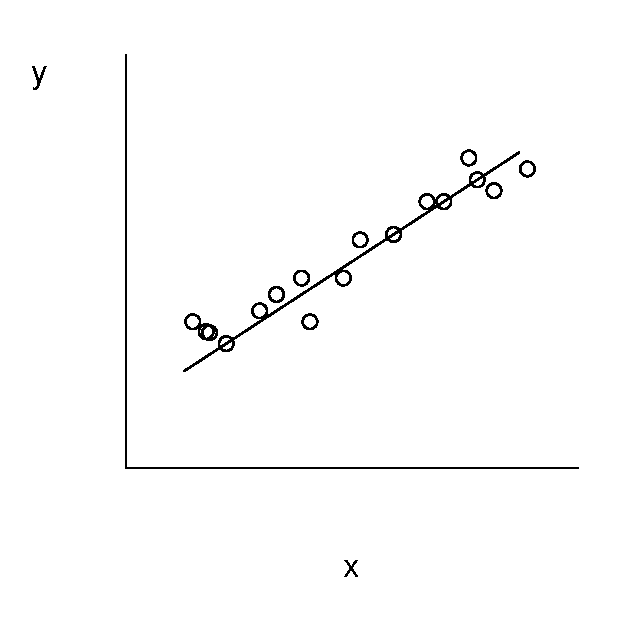
\includegraphics[height=1.8in,width=1.8in]{Chapter2/F2BasicLSRE2.eps} \hfill
    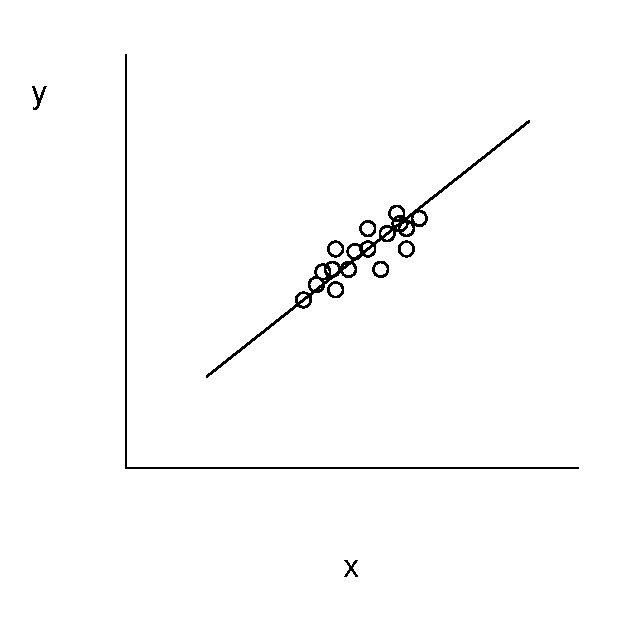
\includegraphics[height=1.8in,width=1.8in]{Chapter2/F2BasicLSRE3.eps} \hfill
    \caption{\label{F2:BasicLSRE} \small These three scatter plots exhibit the same linear
relationship between $y$ and $x$. The plot on the left exhibits
greater variability about the line than the plot in the middle. The
plot on the right exhibits a smaller standard deviation in $x$ than
the plot in the middle.}
  \end{center}
\end{figure}

\bigskip

Equation (\ref{weightb1}) also implies that the regression
coefficient $b_1 $ is normally distributed. That is, recall from
mathematical statistics that linear combinations of normal random
variables are also normal. Thus, if Assumption F5 holds, then $b_1$
is normally distributed. Moreover, several versions of central limit
theorems exists for weighted sums (see, for example, Serfling,
1980). Thus, as discussed in Section 1.4, if the responses $y_i$\
are even approximately normally distributed, then it will be
reasonable to use a normal approximation for the sampling
distribution of $b_1$. Using $se(b_1)$ as the estimated standard
deviation of $b_1$, for large values of $n$ we have that $\left(
b_1-\beta_1\right) /se(b_1)$ has an approximate standard normal
distribution. Although we will not prove it here, under Assumption
F5 $\left( b_1-\beta_1\right) /se(b_1)$\ follows a $t $-distribution
with degrees of freedom $df=n-2$.\index{theorems!central limit}

\section{Statistical Inference}

Having fit a model with a data set, we can make a number of important
statements. Generally, it is useful to think about these statements in three
categories: (i) tests of hypothesized ideas, (ii) estimates of model
parameters and (ii) predictions of new outcomes.

\subsection{Is the Explanatory Variable Important?: The
\textit{t}-Test}\index{hypothesis test!$t$-test}

We respond to the question of whether the explanatory variable is
important by investigating whether or not $\beta_1=0$. The logic is
that if $\beta_1=0$, then the basic linear regression model no
longer includes an explanatory variable $x$. Thus, we translate our
question of the importance of the explanatory variable into a
narrower question that can be answered using the hypothesis testing
framework. This narrower question is, is $ H_0:\beta_1=0$ valid? We
respond to this question by looking at the test statistic:

\begin{center}

\boxedjed
\begin{equation*}
t-\mathrm{ratio}=\frac{\mathrm{estimator-hypothesized~value~of~parameter}}
{\mathrm{standard~error~of~the~estimator}}.
\end{equation*}

\end{boxedminipage}
\end{center}

\index{symbols!$t(b)$, $t$-ratio for $b$}
\index{symbols!$t_{n-2,1-\alpha /2}$, a 1-$\alpha/2$ percentile from
the $t$-distribution with $n-2$ degrees of freedom}

\marginparjed{Appendix A3.3 provides additional details about the
$t$-distribution, including a graph and distribution table.}

For the case of $H_0:\beta_1=0$ , we examine $t$-ratio $
t(b_1)=b_1/se(b_1)$ because the hypothesized value of $\beta_1$\ is
0. This is the appropriate standardization because, under the null
hypothesis and the model assumptions described in Section 2.4, the
sampling distribution of $t(b_1)$ can be shown to be the
$t$-distribution with $ df=n-2$ degrees of freedom. Thus, to test
the null hypothesis $H_0$ against the alternative $H_{a}:\beta_1\neq
0$, we reject $H_0$ if favor of $H_{a}$ if $|t(b_1)|$ exceeds a
$t$-value. Here, this $t$-value is a percentile from the
$t$-distribution using $df=n-2$ degrees of freedom. \ We denote the
significance level as $\alpha $ \ and this $t$-value as
$t_{n-2,1-\alpha /2}$.\index{distributions!t-@{$t-$}}

\linejed

\textbf{Example: Lottery Sales - Continued.} For the lottery sales
example, the residual standard deviation is $s=3,792$. From Table
\ref{T2:SummaryStats}, we have $s_x = 11,098$. Thus, the standard
error of the slope is $se(b_1) = 3792/(11098\sqrt{50-1})=0.0488$.
From Section 2.1, the slope estimate is $b_1=0.647$. Thus, the
$t$-statistic is $t(b_1) = 0.647/0.0488 = 13.4$. We interpret this
by saying that the slope is 13.4 standard errors above zero. For the significance level,
we use the customary value of
$\alpha $ = 5\%. The 97.5th percentile from a $t$-distribution with
$df=50-2=48$ degrees of freedom is $t_{48,0.975}=2.011$. Because
$|13.4|>2.011$, we reject the null hypothesis that the slope
$\beta_1 = 0$ in favor of the alternative that $\beta_1 \neq 0$.

\linejed

\bigskip

\index{symbols!$H_0$, null hypothesis}\index{symbols!$H_a$,
alternative hypothesis}

Making decisions by comparing a $t$-ratio to a $t$-value is called a
$t$ \emph{-test}. Testing $H_0:\beta_1=0$ versus $H_{a}:\beta_1\neq
0$ is just one of many hypothesis tests that can be performed,
although it is the most common. Table \ref{T2:DecMakingProc}
outlines alternative decision-making procedures. These procedures
are for testing $H_0:\beta_1 = d$ where $d$ is a user-prescribed
value that may be equal to zero or any other known value. For
example, in our Section 2.7 example, we will use $d=1$ to test
financial theories about the stock market.


\begin{table}[h]
\caption{\label{T2:DecMakingProc} Decision-Making Procedures for
Testing $H_0:\beta_1 = d$}

\begin{tabular}{cc}
\hline Alternative Hypothesis ($H_{a}$) & Procedure: Reject $H_0$ in
favor of $ H_{a}$ if \\ \hline
$\beta_1>d$ & $t-\mathrm{ratio}>t_{n-2,1-\alpha }$. \\
$\beta_1<d$ & $t-\mathrm{ratio}<-t_{n-2,1-\alpha }$. \\
$\beta_1\neq d$ & $|t-\mathrm{ratio}\mathit{|}>t_{n-2,1-\alpha /2}$. \\
\hline \multicolumn{2}{l}{Notes: The significance level is
$\alpha $. Here, $t_{n-2,1-\alpha }$ is the (1-$\alpha $)th percentile}\\
\multicolumn{2}{l}{~~from the $t$-distribution using $df=n-2$
degrees
of freedom.} \\
\multicolumn{2}{l}{~~The test statistic is $t-\mathrm{ratio} = (b_1
-d)/se(b_1) $.} \\
 \hline
\end{tabular}

\end{table}

Alternatively, one can construct probability ($p$-) values and
compare these to given significant levels. The $p$-value is a useful
summary statistic for the data analyst to report since it allows the
report reader to understand the strength of the deviation from the
null hypothesis. Table \ref{T2:PvalueProc} summarizes the procedure
for calculating $p$-values.

\index{symbols!$p$-value, probability value}

\begin{table}[h]
\caption{\label{T2:PvalueProc} Probability Values for Testing
$H_0:\beta_1 = d$}
\begin{tabular}{cccc}
\hline
Alternative &  &  &  \\
Hypothesis ($H_a$) & $\beta_1>d$ & $\beta_1<d$ & $\beta_1\neq d$
\\ \hline
$p$-value & Pr($t_{n-2}>t-\mathrm{ratio}$) &
Pr($t_{n-2}<t-\mathrm{ratio}$) & $\mathrm{Pr}
(|t_{n-2}|>|t-\mathrm{ratio}\mathit{|})$ \\
\hline \multicolumn{4}{l}{Notes: Here, $t_{n-2}$
is a $t$-distributed random variable with $df=n-2$ degrees } \\
\multicolumn{4}{l}{~~of freedom. The test statistic is
$t-\mathrm{ratio} = (b_1 -d)/se(b_1) $.} \\
\hline
\end{tabular}
\end{table}

Another interesting way of addressing the question of the importance
of an explanatory variable is through the correlation coefficient.
Remember that the correlation coefficient is a measure of linear
relationship between $x$ and $y$. Let's denote this statistic by
$r(y,x)$. This quantity is unaffected by scale changes in either
variable. For example, if we multiply the $x$ variable by the number
$b_1$, then the correlation coefficient remains unchanged. Further,
correlations are unchanged by additive shifts. Thus, if we add a
number, say $b_0$, to each $x$ variable, then the correlation
coefficient remains unchanged. Using a scale change and an additive
shift on the $x$ variable can be used to produce the fitted value $
\widehat{y}=b_0+b_1x$. Thus, using notation, we have $r(y,x)=r(y,
\widehat{y}).$ We may thus interpret the correlation between the
responses and the explanatory variable to be equal to the
correlation between the responses and the fitted values. This leads
then to the following interesting algebraic fact, $R^2=r^2.$ That
is, the coefficient of determination equals the correlation
coefficient squared. This is much easier to interpret if one thinks
of $r$ as the correlation between observed and fitted values. See
Exercise 2.\ref{Ex:Chap2Corr} for steps useful in confirming this
result.

\marginparjed{\large{$R^2=r^2$}}

\subsection{Confidence Intervals}\index{confidence interval}

Investigators often cite the formal hypothesis testing mechanism to
respond to the question ``Does the explanatory variable have a real
influence on the response?'' A natural follow-up question is ``To
what extent does $x$ affect $y$?'' To a certain degree, one could
respond using the size of the $t$-ratio or the $p$-value. However,
in many instances a \emph{confidence interval} for the slope is more
useful.

To introduce confidence intervals for the slope, recall that $b_1$
is our point estimator of the true, unknown slope $\beta_1$. Section
2.4 argued that this estimator has standard error $se(b_1)$ and that
$\left( b_1-\beta_1\right) /se(b_1)$ follows a $t$-distribution with
$n-2$ degrees of freedom. Probability statements can be inverted to
yield confidence intervals. Using this logic, we have the following
confidence interval for the slope $\beta_1$.

\bigskip

\boxedjed

\textit{Definition}. A $100(1-\alpha)$\% confidence interval for the
slope $\beta_1$ is
\begin{equation}\label{E2:ConfIntb1}
b_1\pm t_{n-2,1-\alpha /2} ~se(b_1).
\end{equation}
\end{boxedminipage}
\bigskip

\noindent As with hypothesis testing, $t_{n-2,1-\alpha /2}$ is the
(1-$ \alpha $/2)th percentile from the $t$-distribution with
$df=n-2$ degrees of freedom. Because of the two-sided nature of
confidence intervals, the percentile is 1 - (1 - confidence level) /
2. In this text, for notational simplicity we generally use a 95\%
confidence interval, so the percentile is 1-(1-.0.95)/2 = 0.975. The
confidence interval provides a range of reliability that measures
the usefulness of the estimate.

In Section 2.1, we established that the least squares slope estimate
for the lottery sales example is $b_1=0.647$. The interpretation is
that if a zip code's population differs by 1,000, then we expect mean
lottery sales to differ by \$647. How reliable is this estimate? It
turns out that $ se(b_1)=0.0488$ and thus an approximate 95\%
confidence interval for the slope is
\begin{equation*}
0.647\pm (2.011)(.0488),
\end{equation*}
or (0.549, 0.745). Similarly, if population differs by 1,000, a 95\%
confidence interval for the expected change in sales is (549, 745).
Here, we use the $t$-value $t_{48,0.975}=2.011$ because there are 48
(= $ n$-2) degrees of freedom and, for a 95\% confidence interval,
we need the 97.5th percentile.

\subsection{Prediction Intervals}

In Section 2.1, we showed how to use least squares estimators to
predict the lottery sales for a zip code, outside of our sample,
having a population of 10,000. Because prediction is such an
important task for actuaries, we formalize the procedure so that it
can be used on a regular basis.

To predict an additional observation, we assume that the level of
explanatory variable is known and is denoted by $x_{\ast}$. For
example, in our previous lottery sales example we used $x_{\ast} =
10,000$. We also assume that the additional observation follows the
same linear regression model as the observations in the sample.

Using our least square estimators, our point prediction is
$\widehat{y}_{\ast} = b_0 + b_1 x_{\ast}$, the height of the fitted
regression line at $x_{\ast}$ We may decompose the prediction error
into two parts:

\begin{center}
\begin{tabular}{ccccc}
$\underbrace{y_{\ast} - \widehat{y}_{\ast}}$ & = &
$\underbrace{\beta_0 - b_0 + \left( \beta_1 - b_1 \right) x_{\ast}}$
& + & $\underbrace{\varepsilon_{\ast}}$ \\
{\small prediction error} & {\small =} & {\small error in estimating
the } &
{\small +} & {\small deviation of the additional } \\
&  & {\small regression line at \textit{x}}$_{\ast}$ &  & {\small
response from its mean}
\end{tabular}
\end{center}

It can be shown that the standard error of the prediction is
\begin{equation*}
se(pred) = s \sqrt{1+\frac{1}{n}+\frac{\left(
x_{\ast}-\overline{x}\right) ^2}{(n-1)s_x^2}}.
\end{equation*}
As with $se(b_1)$, the terms $n^{-1}$ and $\left(
x_{\ast}-\overline{x} \right) ^2/\left[ (n-1)s_x^2\right] $\ become
close to zero as the sample size $n$ becomes large. Thus, for large
$n$, we have that $se(pred)\approx s$, reflecting that the error in
estimating the regression line at a point becomes negligible and
deviation of the additional response from its mean becomes the
entire source of uncertainty.\index{symbols!$se(pred)$, standard
error of a prediction}

\bigskip

\boxedjed

\textit{Definition}. A $100(1-\alpha)$\% prediction interval at
$x_{\ast}$ is
\begin{equation}\label{E2:predinteval}
\widehat{y}_{\ast} \pm t_{n-2,1-\alpha /2} ~se(pred)
\end{equation}
where the $t$-value $t_{n-2,1-\alpha /2}$ is the same as used for
hypothesis testing and the confidence interval.
\end{boxedminipage}
\bigskip

\noindent For example, the point prediction at $x_{\ast} = 10,000$
is $\widehat{y}_{\ast}$= 469.7 + 0.647 (10000) = 6,939.7. The
standard error of this prediction is
\begin{equation*}
se(pred) = 3,792 \sqrt{1+\frac{1}{50} + \frac{\left(
10,000-9,311\right)^2}{(50-1)(11,098)^2}} = 3,829.6.
\end{equation*}
With a $t$-value equal to 2.011, this yields an approximate 95\%
prediction interval
\begin{equation*}
6,939.7 \pm (2.011)(3,829.6) = 6,939.7 \pm 7,701.3 = (-761.6,
~14,641.0).
\end{equation*}
We interpret these results by first pointing out that our best
estimate of lottery sales for a zip code with a population of 10,000
is \$6,939.70. Our 95\% prediction interval represents a range of
reliability for this prediction. If we could see many zip codes,
each with a population of 10,000, on average we expect about 19 out
of 20, or 95\%, would have lottery sales between 0 and \$14,641. It
is customary to truncate the lower bound of the prediction interval
to zero if negative values of the response are deemed to be
inappropriate.

\section{Building a Better Model: Residual Analysis}\label{S2:ResidualAnalsis}

Quantitative disciplines calibrate models with data. Statistics
takes this one step further, using discrepancies between the
assumptions and the data to improve model specification. We will
examine the Section 2.2 modeling assumptions in light of the data
and use any mismatch to specify a better model; this process is
known as \textit{diagnostic checking} (like when you go to a doctor
and he or she performs diagnostic routines to check your
health).\index{diagnostic checking!residual analysis}


\index{residual!analysis|see{diagnostic checking}}

\marginparjed{Statistics uses discrepancies between the assumptions
and the data to improve model specification.}

We will begin with the Section 2.2 error representation. Under this
set of assumptions, the deviations \{$\varepsilon _i$\} are
identically and independently distributed (i.i.d), and under
assumption F5, normally distributed. To assess the validity of these
assumptions, one uses (observed) residuals \{$e_i$\} as
approximations for the (unobserved) deviations \{$\varepsilon _i$\}.
The basic theme is that if the residuals are related to a variable
or display any other recognizable pattern, then we should be able to
take advantage of this information and improve our model
specification. The residuals should contain little or no information
and represent only natural variation from the sampling that cannot
be attributed to any specific source. \emph{Residual analysis} is
the exercise of checking the residuals for patterns.

\marginparjed{If the residuals are related to a variable or display
any other recognizable pattern, then we should be able to take
advantage of this information and improve our model specification.}

There are five types of model discrepancies that analysts commonly look for.
If detected, the discrepancies can be corrected with the appropriate
adjustments in the model specification.

\bigskip

\boxedjed

\textbf{Model Misspecification Issues}

\begin{enumerate}
\item \textbf{Lack of Independence}. There may exist relationships among the
deviations \{$\varepsilon _i$\} so that they are not independent.

\item \textbf{Heteroscedasticity}. Assumption E3 that indicates that all
observations have a common (although unknown) variability, known as
\emph{homoscedasticity}. \emph{Heteroscedascity} is the term used
when the variability varies by
observation.\index{heteroscedasticity}\index{homoscedasticity}

\item \textbf{Relationships between Model Deviations and Explanatory Variables}.
If an explanatory variable has the ability to help explain the
deviation $\varepsilon $, then one should be able to use this
information to better predict $y$.

\item \textbf{Nonnormal Distributions}. If the distribution of the deviation
represents a serious departure from normality, then the usual
inference procedures are no longer valid.

\item \textbf{Unusual Points}. Individual observations may have a large
effect on the regression model fit, meaning that the results may be
sensitive to the impact of a single observation.
\end{enumerate}

\end{boxedminipage}
\bigskip

This list will serve the reader throughout your study of regression
analysis. Of course, with only an introduction to basic models we
have not yet seen alternative models that might be used when we
encounter these model discrepancies. In this book's Part II on time
series models, we will study lack of independence among data ordered
over time. Chapter 5 will consider heteroscedasticity in further
detail. The introduction to multiple linear regression in Chapter 3
will be our first look at handling relationships between
\{$\varepsilon _i$\} and additional explanatory variables. We have,
however, already had an introduction to the effect of normal
distributions, seeing that $qq$ plots can detect non-normality and
that transformations can help induce approximate normality. In this
section, we discuss the effects of unusual points.

Much of residual analysis is done by examining a \emph{standardized
residual}, a residual divided by its standard error. An approximate
standard error of the residual is $s$; in Chapter 3 we will give a
precise mathematical definition. There are two reasons why we often
examine standardized residuals in lieu of basic residuals. First, if
responses are normally distributed, then standardized residuals are
approximately realizations from a standard normal distribution. This
provides a reference distribution to compare values of standardized
residuals. For example, if a standardized residual exceeds two in
absolute value, this is considered unusually large and the
observation is called an \emph{outlier}. Second, because
standardized residuals are dimensionless, we get carryover of
experience from one data set to another. This is true regardless of
whether or not the normal reference distribution is applicable.

\subsubsection*{Outliers and High Leverage
Points}\index{leverage}\index{residual!outlier}

Another important part of residual analysis is the identification of
unusual observations in a data set. Because regression estimates are
weighted averages with weights that vary by observation, some
observations are more important than others. This weighting is more
important than many users of regression analysis realize. In fact,
the example below demonstrates that a single observation can have a
dramatic effect in a large data set.

There are two directions in which a data point can be unusual, the
horizontal and vertical directions. By ``unusual,'' we mean that an
observation under consideration seems to be far from the majority of
the data set. An observation that is unusual in the vertical
direction is called an \emph{outlier}. An observation that is
unusual in the horizontal directional is called a \emph{high
leverage point}. An observation may be both an outlier and a high
leverage point.

\linejed

\empexjed{OutlierExample}\index{datasets!outliers and high leverage
points}

\textbf{Example: Outliers and High Leverage Points. }Consider the
fictitious data set of 19 points plus three points, labeled A, B,
and C, given in Figure \ref{F2:Outlier} and Table \ref{T2:Outliers}.
Think of the first 19 points as ``good'' observations that represent
some type of phenomena. We want to investigate the effect of adding
a single aberrant point.


\begin{table}[h]
\caption{\label{T2:Outliers} 19 Base Points Plus Three Types of
Unusual Observations}

\begin{tabular}{c|cccccccccc|ccc}
\hline Variables & \multicolumn{10}{|c|}{19 Base Points} & A & B & C
\\ \hline $x$ & 1.5 & 1.7 & 2.0 & 2.2 & 2.5 & 2.5 & 2.7 & 2.9 & 3.0
& 3.5 & 3.4 & 9.5
& 9.5 \\
$y$ & 3.0 & 2.5 & 3.5 & 3.0 & 3.1 & 3.6 & 3.2 & 3.9 & 4.0 & 4.0 & 8.0 & 8.0
& 2.5 \\ \hline
$x$ & 3.8 & 4.2 & 4.3 & 4.6 & 4.0 & 5.1 & 5.1 & 5.2 & 5.5 &  &  &  &  \\
$y$ & 4.2 & 4.1 & 4.8 & 4.2 & 5.1 & 5.1 & 5.1 & 4.8 & 5.3 &  &  &  &  \\
\hline
\end{tabular}

\end{table}

\begin{figure}[htp]
  \begin{center}
    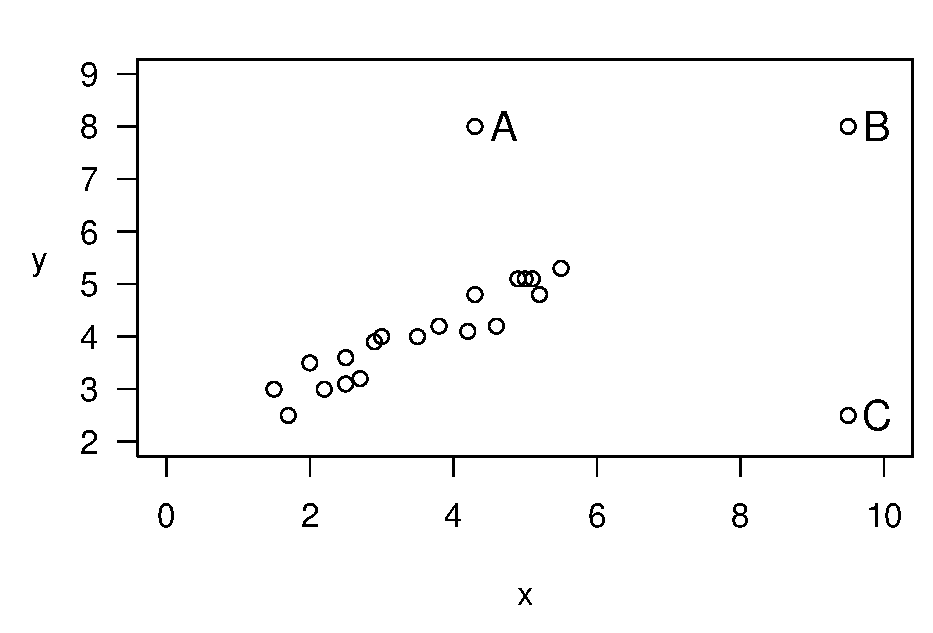
\includegraphics[width=0.6\textwidth]{Chapter2/F2Outlier.eps}
    \caption{\label{F2:Outlier} \small Scatterplot of 19 base plus three unusual points, labeled A, B and C.}
  \end{center}
\end{figure}

To investigate the effect of each type of aberrant point, Table
\ref{T2:OutlierRegression} summarizes the results of four separate
regressions. The first regression is for the nineteen base points.
The other three regressions use the nineteen base points plus each
type of unusual observation.

\begin{table}[h]
\caption{\label{T2:OutlierRegression} Results from Four Regressions}
\begin{tabular}{l|rrrrr}
\hline Data & $b_0$ & $b_1$ & $s$ & $R^2(\%)$ & $t(b_1)$ \\
\hline
19 Base Points & 1.869 & 0.611 & 0.288 & 89.0 & 11.71 \\
19 Base Points ~+~ A & 1.750 & 0.693 & 0.846 & 53.7 & 4.57 \\
19 Base Points ~+~ B & 1.775 & 0.640 & 0.285 & 94.7 & 18.01 \\
19 Base Points ~+~ C & 3.356 & 0.155 & 0.865 & 10.3 & 1.44 \\
\hline
\end{tabular}

\end{table}


Table \ref{T2:OutlierRegression} shows that a regression line
provides a good fit for the nineteen base points. The coefficient of
determination, $R^2$, indicates about 89\% of the variability has
been explained by the line. The size of the typical error, $s$, is
about 0.29, small compared to the scatter in the $y$-values.
Further, the $t$-ratio for the slope coefficient is large.

When the outlier point A is added to the nineteen base points, the
situation deteriorates dramatically. The $R^2$ drops from 89\% to
53.7\% and $s$ increases from about 0.29 to about 0.85. The fitted
regression line itself does not change that much even though our
confidence in the estimates has decreased.

An outlier is unusual in the $y$-value, but ``unusual in the
$y$-value'' depends on the $x$-value. To see this, keep the
$y$-value of Point A the same, but increase the $x$-value and call
the point B.

When the point B is added to the nineteen base points, the
regression line provides a \emph{better} fit. Point B is close to
being on the line of the regression fit generated by the nineteen
base points. Thus, the fitted regression line and the size of the
typical error, $s$, do not change much. However, $R^2$ increases
from 89\% to nearly 95 percent. If we think of $ R^2$ as
$1-(Error~SS)/(Total~SS)$, by adding point B we have increased $
Total~SS$, the total squared deviations in the $y$'s, even though
leaving $ Error~SS$ relatively unchanged. Point B is not an outlier,
but it is a high leverage point.

To show how influential this point is, drop the $y$-value
considerably and call this the new point C. When this point is added
to the nineteen base points, the situation deteriorates
dramatically. The $R^2$ coefficient drops from 89\% to 10\%, and the
$s$ more than triples, from 0.29 to 0.87. Further, the regression
line coefficients change dramatically.

Most users of regression at first do not believe that one point in twenty
can have such a dramatic effect on the regression fit. The fit of a
regression line can always be improved by removing an outlier. If the point
is a high leverage point and not an outlier, it is not clear whether the fit
will be improved when the point is removed.

\linejed

Simply because you can dramatically improve a regression fit by
omitting an observation does not mean you should always do so! The
goal of data analysis is to understand the information in the data.
Throughout the text, we will encounter many data sets where the
unusual points provide some of the most interesting information
about the data. The goal of this subsection is to recognize the
effects of unusual points; Chapter 5 will provide options for
handling unusual points in your analysis.

All quantitative disciplines, such as accounting, economics, linear
programming, and so on, practice the art of \emph{sensitivity analysis}.
Sensitivity analysis is a description of the global changes in a system due
to a small local change in an element of the system. Examining the effects
of individual observations on the regression fit is a type of sensitivity
analysis.

\newpage

\linejed

\textbf{Example: Lottery Sales -- Continued.} Figure
\ref{F2:PlotWithKenosha} exhibits an outlier; the point in the upper
left-hand side of the plot represents a zip code that includes
Kenosha, Wisconsin. Sales for this zip code are unusually high given
its population. Kenosha is close to the Illinois border; residents
from Illinois probably participate in the Wisconsin lottery thus
effectively increasing the potential pool of sales in Kenosha. Table
\ref{T2:RegressionKenosha} summarizes the regression fit both with
and without this zip code.

\begin{table}[h]
\caption{\label{T2:RegressionKenosha} Regression Results with and
without Kenosha}

\begin{tabular}{l|rrrrr}
 \hline
Data & $b_0$ & $b_1$ & $s$ & $R^2(\%)$ & $t(b_1)$ \\ \hline
With Kenosha & 469.7 & 0.647 & 3,792 & 78.5 & 13.26 \\
Without Kenosha & -43.5 & 0.662 & 2,728 & 88.3 & 18.82 \\ \hline
\end{tabular}

\end{table}

\begin{figure}[htp]
  \begin{center}
    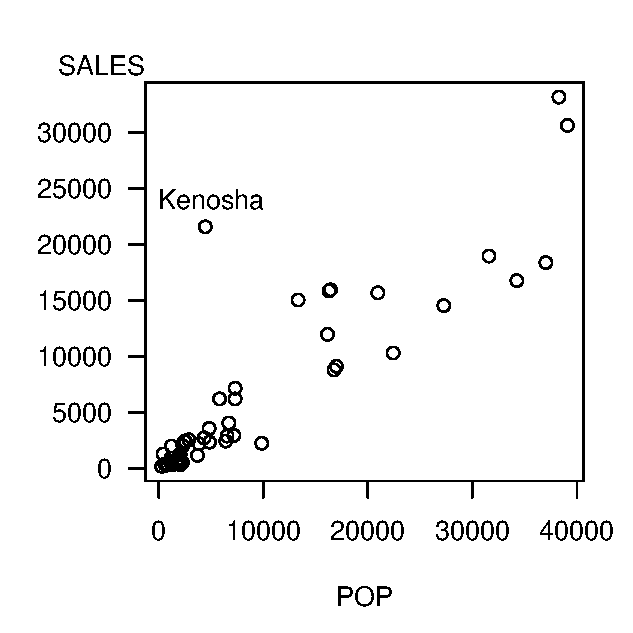
\includegraphics[width=0.6\textwidth]{Chapter2/F2PlotWithKenosha.eps}
    \caption{\label{F2:PlotWithKenosha} \small Scatter plot
of SALES versus POP, with the outlier corresponding to Kenosha
marked.}
  \end{center}
\end{figure}

For the purposes of inference about the slope, the presence of
Kenosha does not alter the results dramatically. Both slope
estimates are qualitatively similar and the corresponding
$t$-statistics are very high, well above cut-offs for statistical
significance. However, there are dramatic differences when assessing
the quality of the fit. The coefficient of determination, $R^2$,
increased from 78.5\% to 88.3\% when deleting Kenosha. Moreover, our
``typical deviation'' $s$ dropped by over \$1,000. This is
particularly important if we wish to tighten our prediction
intervals.

To check the accuracy of our assumptions, it is also customary to
check the normality assumption. One way of doing this is the $qq$
plot, introduced in Section 1.2. The two panels in Figures
\ref{F2:QQplotsKenosha} are $qq$ plots with and without the Kenosha
zip code. Recall that points ``close'' to linear indicate
approximate normality. In the right-hand panel of Figure
\ref{F2:QQplotsKenosha}, the sequence does appear to be linear so
that residuals are approximately normally distributed. This is not
the case in the left-hand panel, where the sequence of points
appears to climb dramatically for large quantiles. The interesting
thing is that the non-normality of the distribution is due to a
single outlier, not a pattern of skewness that is common to all the
observations.

\begin{figure}[htp]
  \begin{center}
    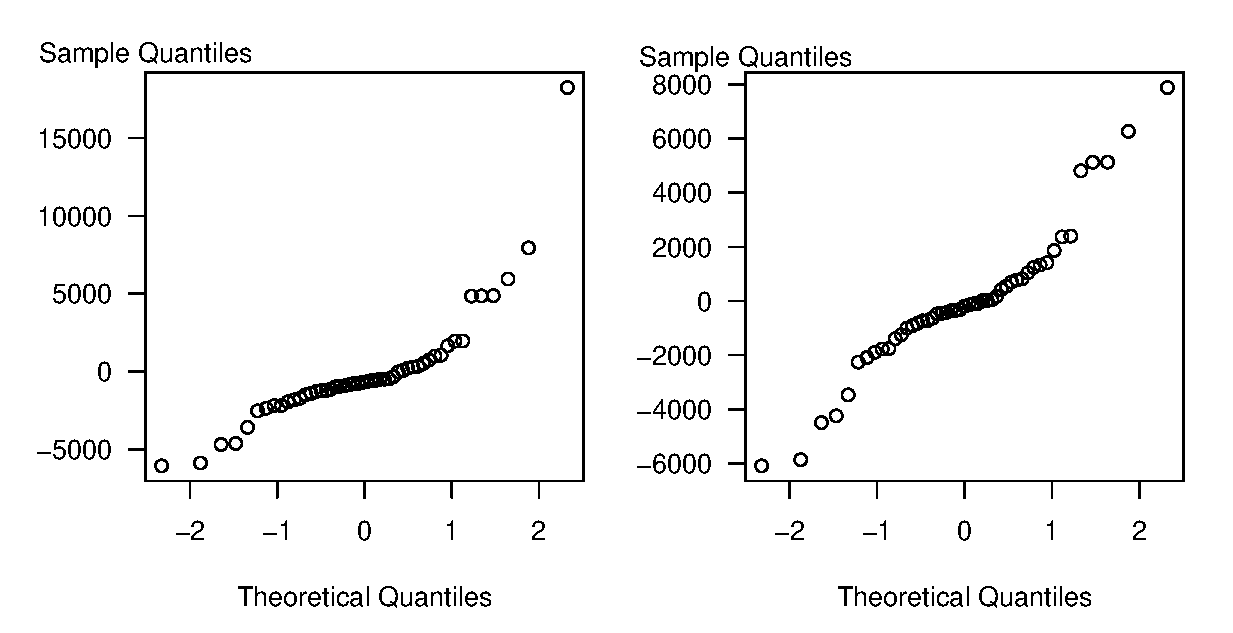
\includegraphics[width=1\textwidth]{Chapter2/F2QQplotsKenosha.eps}
    \caption{\label{F2:QQplotsKenosha} \small $qq$ Plots of Wisconsin Lottery Residuals.
    The left-hand panel is based on all 50 points.
The right-hand panel is based on 49 points, residuals from a
regression after removing Kenosha.}
  \end{center}
\end{figure}

\linejed

\section{Application: Capital Asset Pricing Model}\label{S2:CAPM}\ecaptionjed{Capital Asset Pricing Model}
\index{actuarial \& financial terms and concepts!capital asset
pricing model, CAPM}

In this section, we study a financial application, the Capital Asset
Pricing Model, often referred to by the acronym CAPM. The name is
something of a misnomer in that the model is really about
\emph{returns} based on capital assets, not the prices themselves.
The types of assets that we examine are equity securities that are
traded on an active market, such as the New York Stock Exchange
(NYSE). For a stock on the exchange, we can relate returns to prices
through the following expression:

\scalefont{0.9}
\begin{equation*}
\mathrm{return=}\frac{\mathrm{
price~at~the~end~of~a~period+dividends-price~at~the~beginning~of~a~period}}{
\mathrm{price~at~the~beginning~of~a~period}}.
\end{equation*}
\scalefont{1.1111}

If we can estimate the returns that a stock generates, then
knowledge of the price at the beginning of a generic financial
period allows us to estimate the value at the end of the period
(ending price plus dividends). Thus, we follow standard practice and
model returns of a security.

An intuitively appealing idea, and one of the basic characteristics
of the CAPM, is that there should be a relationship between the
performance of a security and the market. One rationale is simply
that if economic forces are such that the market improves, then
those same forces should act upon an individual stock, suggesting
that it also improve. As noted above, we measure performance of a
security through the return. To measure performance of the market,
several market indices exist that summarize the performance of each
exchange. We will use the ``equally-weighted'' index of the Standard
\& Poor's 500. The Standard \& Poor's 500 is the collection of the
500 largest companies traded on the NYSE, where ``large'' is
identified by Standard \& Poor's, a financial services rating
organization. The equally-weighted index is defined by assuming a
portfolio is created by investing one dollar in each of the 500
companies.

Another rationale for a relationship between security and market
returns comes from financial economics theory. This is the CAPM
theory, attributed to Sharpe (1964) and Lintner (1965) and based on
the portfolio diversification ideas of Harry Markowitz (1959). Other
things equal, investors would like to select a return with a high
expected value and low standard deviation, the latter being a
measure of risk. One of the desirable properties about using
standard deviations as a measure of riskiness is that it is
straight-forward to calculate the standard deviation of a portfolio.
One only needs to know the standard deviation of each security and
the correlations among securities. A notable security is a risk-free
one, that is, a security that theoretically has a zero standard
deviation. Investors often use a 30-day U.S. Treasury bill as an
approximation of a risk-free security, arguing that the probability
of default of the U.S. government within 30 days is negligible.
Positing the existence of a risk-free asset and some other mild
conditions, under the CAPM theory there exists an efficient frontier
called the \emph{securities market line}. This frontier specifies
the minimum expected return that investors should demand for a
specified level of risk. To estimate this line, we can use the
equation\index{actuarial \& financial terms and concepts!securities
market line}
\begin{equation*}
\mathrm{E}~r = \beta_0 + \beta_1 r_m
\end{equation*}
where $r$ is the security return and $r_m$ is the market return. We
interpret $\beta_1 r_m$ as a measure of the amount of security
return that is attributed to the behavior of the market.

Testing economic theory, or models arising from any discipline, involves
collecting data. The CAPM theory is about ex-ante (before the fact) returns
even though we can only test with ex-post (after the fact) returns. Before
the fact, the returns are unknown and there is an entire distribution of
returns. After the fact, there is only a single realization of the security
and market return. Because at least two observations are required to
determine a line, CAPM models are estimated using security and market data
gathered over time. In this way, several observations can be made. For the
purposes of our discussions, we follow standard practice in the securities
industry and examine monthly prices.

\subsubsection*{Data}

\empexjed{CAPM}\index{datasets!capital asset pricing model}

To illustrate, consider monthly returns over the five year period
from January, 1986 to December, 1990, inclusive. Specifically, we
use the security returns from the Lincoln National Insurance
Corporation as the dependent variable ($y$) and the market returns
from the index of the Standard \& Poor's 500 Index as the
explanatory variable ($x$). At the time, the Lincoln was a large,
multi-line, insurance company, headquartered in the midwest of the
U.S., specifically in Fort Wayne, Indiana. Because it was well known
for its' prudent management and stability, it is a good company to
begin our analysis of the relationship between the market and an
individual stock.

We begin by interpreting some of basic summary statistics, in Table
\ref{T2:SumStatsCAPM}, in terms of financial theory. First, an
investor in the Lincoln will be concerned that the five year average
return, $\overline{y}=0.00510$, is below the return of the market,
$\overline{x}=0.00741$. Students of interest theory recognize that
monthly returns can be converted to an annual basis using geometric
compounding. For example, the annual return of the Lincoln is
$(1.0051)^{12}-1=0.062946$, or roughly 6.29 percent. This is
compared to an annual return of 9.26\% (= (1$00((1.00741)^{12}-1$))
for the market. A measure of risk, or volatility, that is used in
finance is the standard deviation. Thus, interpret $s_y$ = 0.0859
$>$ 0.05254 = $s_x$ to mean that an investment in the Lincoln is
riskier than that of the market. Another interesting aspect of Table
\ref{T2:SumStatsCAPM} is that the smallest market return, -0.22052,
is 4.338 standard deviations below its average
((-0.22052-0.00741)/0.05254 = -4.338). This is highly unusual with
respect to a normal distribution.

\begin{table}[h]
\caption{\label{T2:SumStatsCAPM} Summary Statistics of 60 Monthly
Observations}
\begin{tabular}{c|ccccc}
\hline
& & & Standard &  \\
&  Mean & Median & Deviation & Minimum & Maximum\\ \hline
LINCOLN & 0.0051 & 0.0075 & 0.0859 & -0.2803 & 0.3147 \\
MARKET & 0.0074 & 0.0142 & 0.0525 & -0.2205 & 0.1275 \\ \hline
\multicolumn{6}{c}{\textit{Source: Center for Research on Security
Prices, University of Chicago}} \\ \hline
\end{tabular}
\end{table}

We next examine the data over time, as is given graphically in
Figure \ref{F2:TimeSeriesPlots}. These are scatter plots of the
returns versus time, called \emph{time series plots}. In Figure
\ref{F2:TimeSeriesPlots}, one can clearly see the smallest market
return and a quick glance at the horizontal axis reveals that this
unusual point is in October, 1987, the time of the well-known market
crash.


\begin{figure}[htp]
  \begin{center}
    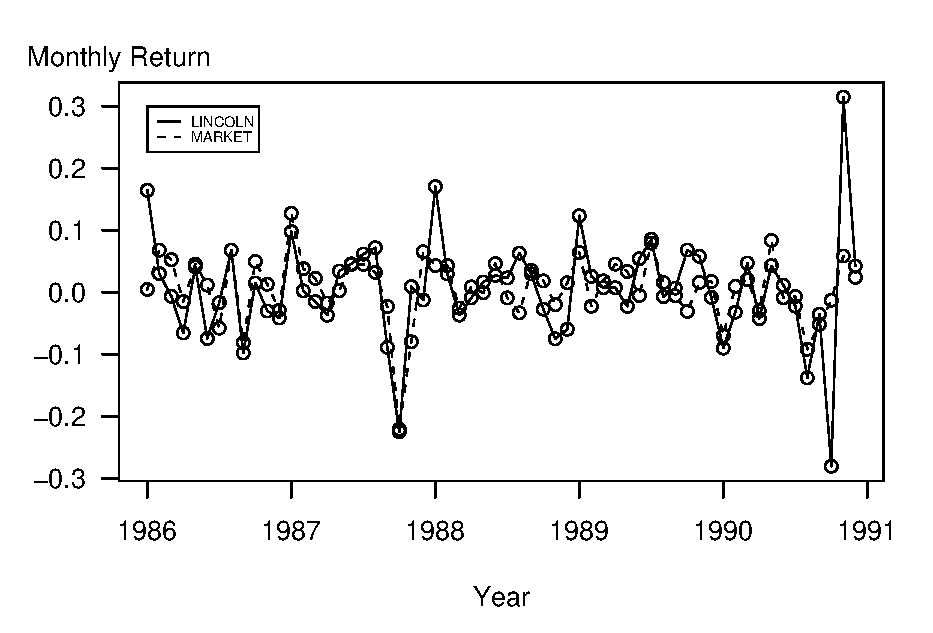
\includegraphics[width=0.8\textwidth]{Chapter2/F2TimeSeriesPlots.eps}
    \caption{\label{F2:TimeSeriesPlots} \small Time series
plot of returns from the Lincoln National Corporation and the
market. There are 60 monthly returns over the period January, 1986
through December, 1990.}
  \end{center}
\end{figure}


\bigskip

The scatter plot in Figure \ref{F2:LincolnvsMarket} graphically
summarizes the relationship between Lincoln's return and the return
of the market. The market crash is clearly evident in Figure
\ref{F2:LincolnvsMarket} and represents a high leverage point. With
the regression line (described below) superimposed, the two outlying
points that can be seen in Figure \ref{F2:TimeSeriesPlots} are also
evident. Despite these anomalies, the plot in Figure
\ref{F2:LincolnvsMarket} does suggest that there is a linear
relationship between Lincoln and market returns.



\begin{figure}[htp]
  \begin{center}
    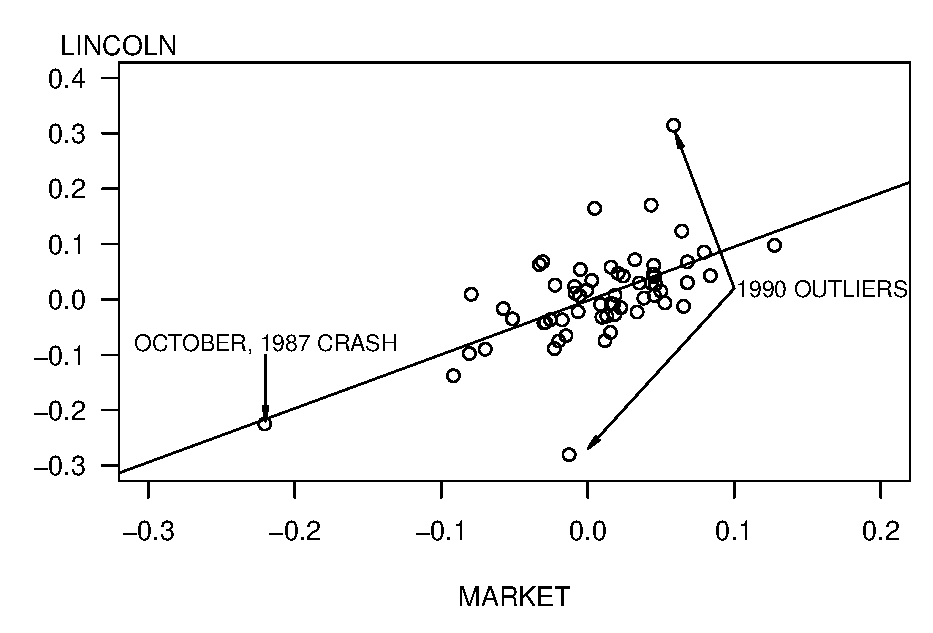
\includegraphics[width=0.8\textwidth]{Chapter2/F2LincolnvsMarket.eps}
    \caption{\label{F2:LincolnvsMarket} \small Scatterplot of Lincoln's return versus the S\&P 500 Index return. The
regression line is superimposed, enabling us to identify the market
crash and two outliers.}
  \end{center}
\end{figure}

\bigskip

\subsubsection*{Unusual Points}

To summarize the relationship between the market and Lincoln's
return, a regression model was fit. The fitted regression is
\begin{equation*}
\widehat{LINCOLN}=-0.00214+0.973 MARKET.
\end{equation*}
The resulting estimated standard error, $s$ = 0.0696 is lower than
the standard deviation of Lincoln's returns, $s_y=0.0859$. Thus, the
regression model explains some of the variability of Lincoln's
returns. Further, the $t$-statistic associated with the slope $b_1$
turns out to be $t(b_1)=5.64$, which is significantly large. One
disappointing aspect is that the statistic $R^2=35.4\%$ can be
interpreted as saying that the market explains only a little over a
third of the variability. Thus, even though the market is clearly an
important determinant, as evidenced by the high $t$-statistic, it
provides only a partial explanation of the performance of the
Lincoln's returns.

In the context of the market model, we may interpret the standard
deviation of the market, $s_x$, as \emph{non-diversifiable risk}.
Thus, the risk of a security can be decomposed into two components,
the diversifiable component and the market component, which is
non-diversifiable. The idea here is that by combining several
securities we can create a portfolio of securities that, in most
instances, will reduce the riskiness of our holdings when compared
with a single security. Again, the rationale for holding a security
is that we are compensated through higher expected returns by
holding a security with higher riskiness. To quantify the relative
riskiness, it is not hard to show that
\begin{equation}
s_y^2 = b_1^2 s_x^2 + s^2 \frac{n-2}{n-1}.
\end{equation}

The riskiness of a security is due to the riskiness due to the
market plus the riskiness due to a diversifiable component. Note
that the riskiness due to the market component, $s_x^2$, is larger
for securities with larger slopes. For this reason, investors think
of securities with slopes $b_1$ greater than one as ``aggressive''
and slopes less than one as ``defensive.''

\subsubsection*{Sensitivity Analysis}

The above summary immediately raises two additional issues. First,
what is the effect of the October, 1987 crash on the fitted
regression equation? We know that unusual observations, such as the
crash, may potentially influence the fit a great deal. To this end,
the regression was re-run without the observation corresponding to
the crash. The motivation for this is that the October 1987 crash
represents a combination of highly unusual events (the interaction
of several automated trading programs operated by the large stock
brokerage houses) that we do not wish to represent using the same
model as our other observations. Deleting this observation, the
fitted regression is
\begin{equation*}
\widehat{LINCOLN} = -0.00181 + 0.956 MARKET,
\end{equation*}
with $R^2=26.4\%$, $t(b_1)=4.52$, $s=0.0702$ and $s_y=0.0811$. We
interpret these statistics in the same fashion as the fitted model
including the October 1987 crash. It is interesting to note,
however, that the proportion of variability explained has actually
\emph{decreased} when excluding the influential point. This serves
to illustrate an important point. High leverage points are often
looked upon with dread by data analysts because they are, by
definition, unlike other observations in the data set and require
special attention. However, when fitting relationships among
variables, they also represent an opportunity because they allow the
data analyst to observe the relationship between variables over
broader ranges than otherwise possible. The downside is that these
relationships may be nonlinear or follow an entirely different
pattern when compared to the relationships observed in the main
portion of the data.

The second question raised by the regression analysis is what can be
said about the unusual circumstances that gave rise to the unusual
behavior of Lincoln's returns in October and November of 1990. A
useful feature of regression analysis is to identify and raise the
question; it does not resolve it. Because the analysis clearly
pinpoints two highly unusual points, it suggests to the data analyst
to go back and ask some specific questions about the sources of the
data. In this case, the answer is straightforward. In October of
1990, the Travelers' Insurance Company, a competitor, announced that
it would take a large write-off in their real estate portfolio. due
to an unprecedented number of mortgage defaults. The market reacted
quickly to this news, and investors assumed that other large stock
life insurers would also soon announce large write-offs.
Anticipating this news, investors tried to sell their portfolios of,
for example, Lincoln's stock, thus causing the price to plummet.
However, it turned out that investors overreacted to this news and
that Lincoln's portfolio of real estate was indeed sound. Thus,
prices quickly returned to their historical levels.

\section{Illustrative Regression Computer Output}

Computers and statistical software packages that perform specialized
calculations play a vital role in modern-day statistical analyses.
Inexpensive computing capabilities have allowed data analysts to
focus on relationships of interest. Specifying models that are
attractive merely for their computational simplicity is much less
important now compared to times before the widespread availability
of inexpensive computing. An important theme of this text is to
focus on relationships of interest and to rely on widely available
statistical software to estimate the models that we specify.

With any computer package, generally the most difficult parts of operating
the package are the (i) input, (ii) using the commands and (iii)
interpreting the output. You will find that most modern statistical software
packages accept spreadsheet or text-based files, making input of data
relatively easy. Personal computer statistical software packages have
menu-driven command languages with easily accessible on-line help
facilities. Once you decide what to do, finding the right commands is
relatively easy.

This section provides guidance in interpreting the output of
statistical packages. Most statistical packages generate similar
output. Below, three examples of standard statistical software
packages, EXCEL, SAS and R are given. The annotation symbol
``\lbrack .]'' marks a statistical quantity that is described in the
legend. Thus, this section provides a link between the notation used
in the text and output from some of the standard statistical
software packages.

\scalefont{0.8}

\bigskip

\noindent \rule{5.5in}{0.03in}

\bigskip

{\textbf{EXCEL Output}}

\begin{alltt}
Regression Statistics
Multiple R              0.886283[F]
R Square                0.785497[k]
Adjusted R Square       0.781028[l]
Standard Error          3791.758[j]
Observations              50[a]

ANOVA
           df              SS          MS             F     Significance F
Regression   1[m]   2527165015 [p]  2527165015 [s]  175.773[u]   1.15757E-17[v]
Residual    48[n]   690116754.8[q]  14377432.39[t]
Total       49[o]   3217281770 [r]

        Coefficients    Standard Error      t Stat         P-value
Intercept    469.7036[b] 702.9061896[d]   0.668230846[f] 0.507187[h]
X Variable 1 0.647095[c] 0.048808085[e]   13.25794257[g] 1.16E-17[i]

\end{alltt}

\noindent \rule{5.5in}{0.03in}

\newpage
\noindent \rule{5.5in}{0.03in}

\bigskip

{\textbf{SAS Output}}

\begin{alltt}
                          The SAS System
                         The REG Procedure
                    Dependent Variable: SALES

                        Analysis of Variance
                               Sum of           Mean
Source                   DF        Squares         Square     F Value      Pr > F
Model                  1[m]   2527165015[p]   2527165015[s]   175.77[u]    <.0001[v]
Error                 48[n]    690116755[q]     14377432[t]
Corrected Total       49[o]   3217281770[r]

        Root MSE           3791.75848[j]    R-Square     0.7855[k]
        Dependent Mean     6494.82900[H]    Adj R-Sq     0.7810[l]
        Coeff Var            58.38119[I]

                        Parameter Estimates
                           Parameter       Standard
Variable     Label        DF     Estimate        Error      t  Value    Pr > |t|
Intercept    Intercept     1   469.70360[b]  702.90619[d]    0.67[f]    0.5072[h]
POP          POP           1     0.64709[c]    0.04881[e]   13.26[g]    <.0001[i]
\end{alltt}

\noindent \rule{5.5in}{0.03in}

\bigskip

{\textbf{R Output}}

\begin{alltt}
Analysis of Variance Table

Response: SALES
          Df     Sum Sq      Mean Sq        F value         Pr(>F)
POP        1[m] 2527165015[p] 2527165015[s] 175.77304[u] <2.22e-16[v]***
Residuals 48[n]  690116755[q]   14377432[t]
---
Call: lm(formula = SALES ~ POP)

Residuals:
   Min     1Q Median     3Q    Max
 -6047  -1461   -670    486  18229

Coefficients:
            Estimate     Std. Error t value     Pr(>|t|)
(Intercept) 469.7036[b] 702.9062[c]  0.67[f]    0.51     [h]
POP           0.6471[c]   0.0488[e] 13.26[g]   <2e-16 ***[i]
---
Signif. codes:  0 �***� 0.001 �**� 0.01 �*� 0.05 �.� 0.1 � � 1

Residual standard error: 3790[j] on 48[n] degrees of freedom
Multiple R-Squared: 0.785[k],      Adjusted R-squared: 0.781[l]
F-statistic:  176[u] on 1[m] and 48[n] DF,  p-value: <2e-16[v]
\end{alltt}

\noindent \rule{5.5in}{0.03in} \scalefont{1.25}



\newpage \textbf{Legend Annotation Definition, Symbol }
\index{symbols!$n$, sample size}\index{symbols!$b_0$, least squares
intercept}\index{symbols!$b_1$, least squares
slope}\index{symbols!$se(b)$, standard error of $b$}
\index{symbols!$t(b)$, $t$-ratio for $b$}\index{symbols!$p$-value,
probability value}\index{symbols!$R^2$, coefficient of
determination} \index{symbols!$s^2$, mean square error}
\index{symbols!$s$, residual standard
deviation}\index{symbols!$R_a^2$, coefficient of determination
adjusted for degrees of freedom}

\begin{multicols}{2}

\scalefont{0.9}

[a] Number of observations $n$.

[b] The estimated intercept $b_0$.

[c] The estimated slope $b_1$.

[d] The standard error of the intercept, $se(b_0)$.

[e] The standard error of the intercept, $se(b_1)$.

[f] The $t$-ratio associated with the intercept, $t(b_0) =
b_0/se(b_0)$.

[g] The $t$-ratio associated with the slope, $t(b_1) = b_1/se(b_1)$.

[h] The $p$-value associated with the intercept; here, $
p-value=Pr(|t_{n-2}|>|t(b_0)|)$, where $t(b_0)$ is the realized
value (0.67 here) and $t_{n-2}$ has a $t$-distribution with
$df=n-2$.

[i] The $p$-value associated with the slope; here, $
p-value=Pr(|t_{n-2}|>|t(b_1)|)$, where $t(b_1)$ is the realized
value (13.26 here) and $t_{n-2}$ has a $t$-distribution with $
df=n-2 $.

[j] The residual standard deviation, $s$.

[k] The coefficient of determination, $R^2$.

[l] The coefficient of determination adjusted for degrees of
freedom, $R_{a}^2$. (This term will be defined in Chapter 3.)

[m] Degree of freedom for the regression component. This is 1 for
one explanatory variable.

[n] Degree of freedom for the error component, $n-2$, for regression
with one explanatory variable.

[o] Total degrees of freedoms, $n-1$.

[p] The regression sum of squares, $Regression~SS$.

[q] The error sum of squares, $Error~SS$.

[r] The total sum of squares, $Total~SS$.

\index{symbols!$Error~SS$, error sum of
squares}\index{symbols!$Regression~SS$, regression sum of
squares}\index{symbols!$Total~SS$, total sum of squares}


[s] The regression mean square, $Regression~MS = Regression~SS/1$,
for one explanatory variable.

[t] The error mean square, $s^2=Error~MS = Error~SS/(n-2)$, for one
explanatory variable.

[u] The $F-ratio=(Regression~MS)/(Error~MS)$. (This term will be defined in
Chapter 3.)

[v] The $p$-value associated with the $F-ratio$. (This term will be defined
in Chapter 3.)

[w] The observation number, $i$.

[x] The value of the explanatory variable for the $i$th observation,
$x_i$.

[y] The response for the $i$th observation, $y_i$.

[z] The fitted value for the $i$th  observation, $\widehat{y}_i$.

[A] The standard error of the fit, $se(\widehat{y}_i)$.

[B] The residual for the $i$th observation, $e_i$.

[C] The standardized residual for the $i$th  observation,
$e_i/se(e_i)$. The standard error $se(e_i)$ will be defined in
Section 5.3.1.

[F] The multiple correlation coefficient is the square root of the
coefficient of determination, $R=\sqrt{R^2}$. This will be defined
in Chapter 3.

[G] The standardized coefficient is $b_1s_x/s_y$ For regression with
one explanatory variable, this is equivalent to $r$, the correlation
coefficient.

[H] The average response, $\overline{y}$.

[I] The coefficient of variation of the response is
$s_y/\overline{y}$. SAS prints out $100s_y/\overline{y}$ .

\scalefont{1.1111}

\end{multicols}


\section{Further Reading and References}

Relatively few applications of regression are basic in the sense
that they use only one explanatory variable; the purpose of
regression analysis is to reduce complex relationships among many
variables. Section \ref{S2:CAPM} described an important exception to
this general rule, the CAPM finance model; see Panjer et al. (1998)
for additional actuarial descriptions of this model. Campbell et al.
(1997) gives a financial econometrics perspective.

\bigskip

\newpage

\textbf{Chapter References}

\begin{multicols}{2}

\scalefont{0.9}

Anscombe, Frank (1973). Graphs in statistical analysis. \textit{The
American Statistician} 27, 17-21.

Campbell, John Y., Andrew W. Lo and A. Craig MacKinlay (1997).
\textit{The Econometrics of Financial Markets}. Princeton University
Press, Princeton, New Jersey.

Frees, Edward W. and Tom W. Miller (2003). Sales forecasting using
longitudinal data models. \textit{International Journal of
Forecasting} 20, 97-111.

Goldberger, Arthur (1991). \textit{A Course in Econometrics}.
Harvard University Press, Cambridge.

Koch, Gary J. (1985). A basic demonstration of the [-1, 1] range for
the correlation coefficient. \textit{American Statistician} 39,
201-202.

Linter, J. (1965). The valuation of risky assets and the selection
of risky investments in stock portfolios and capital budgets.
\textit{Review of Economics and Statistics}, 13-37.

Manistre, B. John and Geoffrey H. Hancock (2005). Variance of the
CTE estimator. \textit{North American Actuarial Journal} 9(2),
129-156.

Markowitz, Harry (1959). \textit{Portfolio Selection: Efficient
Diversification of Investments}. John Wiley, New York.

Panjer, Harry H., Phelim P. Boyle, Samuel H. Cox, Daniel Dufresne,
Hans U. Gerber, Heinz H. Mueller, Hal W. Pedersen, Stanley R.
Pliska, Michael Sherris, Elias S. Shiu and Ken S. Tan (1998).
\textit{Financial Economics: With Applications to Investment,
Insurance and Pensions}. Society of Actuaries, Schaumburg, Illinois.

Pearson, Karl (1895). \textit{Royal Society Proceedings} 58, 241.

Serfling, Robert J. (1980). \textit{Approximation Theorems of
Mathematical Statistics}. John Wiley and Sons, New York.

Sharpe, William F. (1964). Capital asset prices: A theory of market
equilibrium under risk. \textit{Journal of Finance}, 425-442.

Stigler, Steven M. (1986). \textit{The History of Statistics:  The
Measurement of Uncertainty before 1900}. Harvard University Press,
Cambridge, MA.

\scalefont{1.1111}

\end{multicols}


\section{Exercises}

\scalefont{0.90}

\begin{exercises}

\subsection*{Sections 2.1-2.2}

\item Consider the following data set~~
\begin{tabular}{l|ccc}
\hline
$i$ & 1 & 2 & 3 \\
$x_i$ & 2 & -6 & 7 \\
$y_i$ & 3 & 4 & 6\\ \hline
\end{tabular}.

Fit a regression line using the method of least squares. Determine
$r$, $b_1$ and $b_0$.

\item \label{Ex:ZeroCorr} \textbf{A perfect relationship, yet zero correlation.} Consider the
quadratic relationship $y=x^2$, with data $
\begin{tabular}{l|rrrrr}
\hline
$i$ & 1 & 2 & 3 & 4 & 5 \\
$x_i$ & -2 & -1 & 0 & 1 & 2 \\
$y_i$ & 4 & 1 & 0 & 1 & 4 \\ \hline
\end{tabular}.$

a. Produce a rough graph for this data set.

b. Check that the correlation coefficient is $r=0$.


\item \textbf{Boundedness of the correlation coefficient.} Use the
following steps to show that $r$ is bounded by -1 and 1 (These steps
are due to Koch, 1990).

a. Let $a$ and $c$ be generic constants. Verify
\begin{eqnarray*}
0 & \leq & \frac{1}{n-1}\sum_{i=1}^{n}\left(
a\frac{x_i-\overline{x}}{s_x}-c
\frac{y_i-\overline{y}}{s_y}\right) ^2 \\
&=& a^2+c^2-2acr.
\end{eqnarray*}

b. Use the results in part (a) to show $2ac(r-1)\leq (a-c)^2.$

c. By taking $a=c$, use the result in part (b) to show $r\leq 1$.

d. By taking $a=-c$, use the results in part (b) to show $r\geq -1$.

e. Under what conditions is $r=-1$? Under what conditions is $r=1$?


\item \textbf{Regression coefficients are weighted sums.} Show that
the intercept term, $b_0$, can be expressed as a weighted sum of the
dependent variables. That is, show that
$b_0=\sum_{i=1}^{n}w_{i,0}y_i.$ Further, express the weights in
terms of the slope weights, $w_i$.

\item \textbf{Another expression for the slope as a weighted sum}

a. Using algebra, establish an alternative expression
\begin{equation*}
b_1=\frac{\sum_{i=1}^{n}weight_i~slope_i}{ \sum_{i=1}^{n}weight_i}.
\end{equation*}
Here, $slope_i$ is the slope between $(x_i,y_i)$ and
$(\bar{x},\bar{y})$. Give a precise form for the weight $weight_i$
as a function of the explanatory variable $x$.

b. Suppose that $\bar{x} = 4,\bar{y} = 3, x_1 = 2 \mathrm{~and~} y_1
= 6$. Determine the slope and weight for the first observation, that
is, $slope_1$ and $weight_1$.


\item Consider two variables, $y$ and $x$. Do a regression
of $y$ on $x$ to get a slope coefficient which we call $b_{1,x,y}$.
Do another regression of $x$ on $y$ to get a slope coefficient which
we call $b_{1,y,x}$. Show that the correlation coefficient between
$x$ and $y$ is the geometric mean of the two slope coefficients up
to sign, that is, show that $|r|=\sqrt{ b_{1,x,y}b_{1,y,x}}.$

\item \textbf{Regression through the origin.} Consider the model
$y_i=\beta_1 x_i + \varepsilon _i$, that is, regression with one
explanatory variable \emph{without} the intercept term. This model
is called \emph{regression through the origin} because the true
regression line $\mathrm{E}y = \beta_1 x$ passes through the origin
(the point (0, 0)). For this model, the least squares estimate of
$\beta_1$ is that number $b_1$ that minimizes the sum of squares
$\mathrm{SS}(b_1^{\ast} )=\sum_{i=1}^{n}\left( y_i -
b_1^{\ast}x_i\right) ^2.$

a. Verify that
\begin{equation*}
b_1 = \frac{\sum_{i=1}^{n} x_i y_i}{\sum_{i=1}^{n}x_i^2}.
\end{equation*}

b. Consider the model $y_i=\beta_1 z_i^2 + \varepsilon _i$, a
quadratic model passing through the origin. Use the result of part
(a) to determine the least squares estimate of $\beta_1$.

\item \label{Ex:SimpleBLR} a. Show that
\begin{equation*}
s_y^2=\frac{1}{n-1}\sum_{i=1}^{n}\left( y_i-\overline{y}\right) ^2=
\frac{1}{n-1}\left( \sum_{i=1}^{n}y_i^2-n\overline{y}^2\right) .
\end{equation*}

b. Follow the same steps to show $\sum_{i=1}^{n}\left( y_i -
\overline{y} \right) \left( x_i-\overline{x}\right) =\sum_{i=1}^{n}
x_i y_i - n \overline{x}~\overline{y}.$

c. Show that
\begin{equation*}
b_{1}=\frac{\sum_{i=1}^{n}\left( y_i-\overline{y}\right) \left( x_i-
\overline{x}\right) }{\sum_{i=1}^{n}\left( x_i - \overline{x}
\right) ^2}
\end{equation*}

d. Establish the commonly used formula
\begin{equation*}
b_{1}=\frac{\sum_{i=1}^{n}x_iy_i-n\overline{x}~\overline{y}}{\sum_{i=1}^{n}x_i^2
- n\overline{x}^2}.
\end{equation*}

\index{categorical variable!binary}
\item \textbf{Interpretation of coefficients associated with a binary
explanatory variable.}\label{Ex:TwoPoPSLR} Suppose that $x_i$ only
takes on the values 0 and 1. Out of the $n$ observations, $n_1$ take
on the value $x=0$. These $n_1 $ observations have an average $y$
value of $\overline{y}_1$. the remaining $n-n_1$ observations have
value $x=1$ and an average $y$ value of $\overline{y}_2$. Use
Exercise 2.\ref{Ex:SimpleBLR} to show that $b_1 = \overline{y}_2 -
\overline{y}_1.$

\newpage

\empexjed{WiscNursingHome}\index{datasets!nursing home utilization}

\item \textbf{Nursing Home Utilization.}\label{Ex:NursHome2a}
This exercise considers nursing home data provided by the Wisconsin
Department of Health and Family Services (DHFS) and described in
Exercise 1.\ref{Ex:NursHome}.

\textbf{Part 1:} Use cost report year 2000 data, and do the
following analysis.

a. Correlations

a(i). Calculate the correlation between TPY and LOGTPY. Comment on
your result.

a(ii). Calculate the correlation among TPY, NUMBED and SQRFOOT. Do
these variables appear highly correlated?

a(iii). Calculate the correlation between TPY and NUMBED/10. Comment
on your result.

b. Scatter plots. Plot TPY versus NUMBED and TPY versus SQRFOOT.
Comment on the plots.

c. Basic linear regression.

c(i). Fit a basic linear regression model using TPY as the outcome
variable and NUMBED as the explanatory variable. Summarize the fit
by quoting the coefficient of determination, $R^2$, and the
$t$-statistic for NUMBED.

c(ii). Repeat c(i), using SQRFOOT instead of NUMBED. In terms of
$R^2$, which model fits better?

c(iii). Repeat c(i), using LOGTPY for the outcome variable and
LOG(NUMBED) as the explanatory variable.

c(iv). Repeat c(iii), using LOGTPY for the outcome variable and
LOG(SQRFOOT) as the explanatory variable.

\textbf{Part 2:} Fit the model in Part 1.c(1) using 2001 data. Are
the patterns stable over time?


\subsection*{Sections 2.3-2.4}

\item Suppose that, for a sample size of $n$ = 3, you have $
e_2$ = 24 and $e_{3}$ = -1. Determine $e_{1}$.

\item Suppose that $r=0$, $n=15$ and $s_y = 10$. Determine
$s$.

\item \textbf{The correlation coefficient and
the coefficient of determination.}\label{Ex:Chap2Corr}  Use the
following steps to establish a relationship between the coefficient
of determination and the correlation coefficient.

a. Show that $\widehat{y}_i-\overline{y}=b_1(x_i-\overline{x}).$

b. Use part (a) to show that $Regress~SS=$ $\sum_{i=1}^{n}\left(
\widehat{y}_i - \overline{y} \right)^2 = b_1^2s_x^2(n-1).$

c. Use part (b) to establish $R^2=r^2.$

\item \label{Ex:AverageResid} Show that the average residual is zero, that is, show
that $n^{-1}\sum_{i=1}^{n} e_i=0.$

\item \textbf{Correlation between residuals and explanatory variables.}
Consider a generic sequence of pairs of numbers ($x_1,y_1$), ...,
($x_n,y_n$) with the correlation coefficient computed as \
$r(y,x)=\left[ (n-1)s_ys_x\right] ^{-1}\sum_{i=1}^{n}\left(
y_i-\overline{y}\right) \left( x_i-\overline{x}\right) .$

a. Suppose that either $\overline{y}=0,\overline{x}=0$ or both
$\overline{x}$ \ and $\overline{y}=0.$ Then, check that $r(y,x)=0$
implies $\sum_{i=1}^{n}y_i x_i=0$\ and vice-versa.

b. Show that the correlation between the residuals and the
explanatory variables is zero. Do this by using part (a) of Exercise
2.13 to show that $\sum_{i=1}^{n} x_i e_i = 0$ and then apply part
(a).

c. Show that the correlation between the residuals and fitted values
is zero. Do this by showing that $\sum_{i=1}^n \widehat{y}_i e_i =
0$ \ and then apply part (a).



\item \textbf{Correlation and $t$-statistics.} Use the following steps to
establish a relationship between the correlation coefficient and the
$t$-statistic for the slope.

a Use algebra to check that
\begin{equation*}
R^2=1-\frac{n-2}{n-1}\frac{s^2}{s_y^2}.
\end{equation*}

b. Use part (a) to establish the following quick computational
formula for $s,$
\begin{equation*}s = s_y \sqrt{(1-r^2)\frac{n-1}{n-2}}.\end{equation*}

c. Use part (b) to show that
\begin{equation*}
t(b_1) = \sqrt{n-2}\frac{r}{\sqrt{1-r^2}}.
\end{equation*}

\subsection*{Sections 2.6-2.7}

\item \textbf{Effects of an unusual point.} You are analyzing a data
set of size $n=100$. You have just performed a regression analysis
using one predictor variable and notice that the residual for the
10th observation is unusually large.

a. Suppose that, in fact, it turns out that $e_{10}=8s$. What
percentage of the error sum of squares, $Error~SS$, is due to the
10th observation?

b. Suppose that $e_{10}=4s$. What percentage of the error sum of
squares, $Error~SS$, is due to the 10th observation?

c. Suppose that you reduce the data set to size $n=20$. After
running the regression, it turns out that we still have $10=4s$.
What percentage of the error sum of squares, $Error~SS$, is due to
the 10th observation?

\item Consider a data set consisting of 20 observations
with the following summary statistics: $\overline{x}=0$,
$\overline{y}=9$, $s_x=1$ and $s_y=10$. You run a regression using
using one variable and determine that $s=7$. Determine the standard
error of a prediction at $x_{\ast}=1.$

\empexjed{AnscombesData}\index{datasets!Anscombe's data}

\item \textbf{Summary statistics can hide important
relationships.} The data in Table \ref{Ex:Anscombes} is due to
Anscombe (1973). The purpose of this exercise is to demonstrate how
plotting data can reveal important information that is not evident
in numerical summary statistics.

\begin{table}[h]
\scalefont{0.80} \caption{\label{Ex:Anscombes} \small Anscombe's
(1973) Data}
\begin{center}
\begin{tabular}{c|rrrrrr}
\hline
obs &  &  &  &  &  &  \\
num & $x_1$ & $y_1$ & $y_2$ & $y_3$ & $x_2$ & $y_4$ \\
\hline 1 & 10 & 8.04 & 9.14 & 7.46 & 8 &
6.58 \\
2 & 8 & 6.95 &  8.14 & 6.77 & 8 &
5.76 \\
3 & 13 & 7.58 & 8.74 & 12.74 & 8 &
7.71 \\
4 & 9 & 8.81 & 8.77 & 7.11 & 8 &
8.84 \\
5 & 11 & 8.33 & 9.26 & 7.81 & 8 &
8.47 \\
6 & 14 & 9.96 & 8.10 & 8.84 & 8 &
7.04 \\
7 & 6 & 7.24 & 6.13 & 6.08 & 8 &
5.25 \\
8 & 4 & 4.26 & 3.10 & 5.39 & 8 &
5.56 \\
9 & 12 & 10.84 & 9.13 & 8.15 & 8 &
7.91 \\
10 & 7 & 4.82 & 7.26 & 6.42 & 8 &
6.89 \\
11 & 5 & 5.68 & 4.74 & 5.73 & 19 & 12.50 \\
\hline
\end{tabular}
\end{center}\scalefont{1.25}\end{table}


a. Compute the averages and standard deviations of each column of
data. Check that the averages and standard deviations of each of the
$x$ columns are the same, within two decimal places, and similarly
for each of the $y$ columns.

b. Run four regressions, (1) $y_{1}$ on $x_{1}$, (2) $y_2$ on
$x_{1}$, (3) $y_{3}$ on $x_{1}$ and (4) $y_{4}$ on $x_2$. Verify,
for each of the four regressions fits, that $b_0\approx 3.0$,
$b_{1}\approx 0.5$, $s\approx 1.237$ and $R^2\approx 0.677$, within
two decimal places.

c. Produce scatter plots for each of the four regression models that
you fit in part (b).

d. Discuss the fact that the fitted regression models produced in
part (b) imply that the four data sets are similar although the four
scatter plots produced in part (c) yield a dramatically different
story.



\bigskip

\empexjed{WiscNursingHome}\index{datasets!nursing home utilization}

\item \textbf{Nursing Home Utilization.}\label{Ex:NursHome2b}
This exercise considers nursing home data provided by the Wisconsin
Department of Health and Family Services (DHFS) and described in
Exercise 1.\ref{Ex:NursHome} and 2.\ref{Ex:NursHome2a}.

You decide to examine the relationship between total patient years
(LOGTPY) and the number of beds (LOGNUMBED), both in logarithmic
units, using cost report year 2001 data.

a. Summary statistics. Create basic summary statistics for each
variable. Summarize the relationship through a correlation statistic
and a scatter plot.

b. Fit the basic linear model. Cite the basic summary statistics,
include the coefficient of determination, the regression coefficient
for LOGNUMBED and the corresponding $t$-statistic.

c. Hypothesis testing. Test the following hypotheses at the 5\ level
of significance using a $t$-statistic. Also compute the
corresponding $p$-value.

c(i). Test $H_0: \beta_1 = 0$ versus $H_a: \beta_1 \neq 0$.

c(ii). Test $H_0: \beta_1 = 1$ versus $H_a: \beta_1 \neq 1$.

c(iii). Test $H_0: \beta_1 = 1$ versus $H_a: \beta_1 > 1$.

c(iv). Test $H_0: \beta_1 = 1$ versus $H_a: \beta_1 < 1$.

d. You are interested in the effect that a marginal change in
LOGNUMBED has on the expected value of LOGTPY.

d(i). Suppose that there is a marginal change in LOGNUMBED of 2.
Provide a point estimate of the expected change in LOGTPY.

d(ii). Provide a 95\% confidence interval corresponding to the point
estimate in part d(i).

d(iii). Provide a 99\% confidence interval corresponding to the
point estimate in part d(i).

e. At a specified number of beds estimate $x_{*} = 100$, do these
things:

e(i). Find the predicted value of LOGTPY.

e(ii). Obtain the standard error of the prediction.

e(iii). Obtain a 95\% prediction interval for your prediction.

e(iv). Convert the point prediction in part e(i) and the prediction
interval obtained in part e(iii) into total person years (through
exponentiation).

e(v). Obtain a prediction interval as in part e(iv), corresponding
to a 90\% level (in lieu of 95\%).


\empexjed{IPO}\index{datasets!initial public
offerings}\index{actuarial \& financial terms and concepts!initial
public offering, IPO}

\item \textbf{Initial Public Offerings.} As a financial analyst, you wish to convince a client of the merits
of investing in firms that have just entered a stock exchange, as an
IPO (initial public offering). Thus, you gather data on 116 firms
that priced during the six-month time frame of January 1, 1998
through June 1, 1998. By looking at this recent historical data, you
are able to compute RETURN, the firm's one-year return (in percent).

You are also interested in looking at financial characteristics of
the firm that may help you understand (and predict) the return. You
initially examine REVENUE, the firm's 1997 revenues in millions of
dollars. Unfortunately, this variable was not available for six
firms. Thus, the statistics below are for the 110 firms that have
both REVENUES and RETURNS. In addition, Table \ref{Ex:IPOSumStats}
provides information on the (natural) logarithmic revenues, denoted
as LnREV, and the initial price of the stock, denoted as PRICEIPO.

\begin{table}[h]
\scalefont{0.80} \caption{\label{Ex:IPOSumStats} \small  Initial
Public Offering Summary Statistics}
\begin{center}
\begin{tabular}{l|rrrrr}
\hline
 & & Standard \\
           & Mean & Median &  Deviation & Minimum & Maximum\\\hline
    RETURN &      0.106 &     -0.130 &      0.824 &     -0.938 &      4.333 \\
       REV &    134.487 &     39.971 &    261.881 &      0.099 &   1455.761 \\
     LnREV &      3.686 &      3.688 &      1.698 &     -2.316 &      7.283 \\
  PRICEIPO &     13.195 &     13.000 &      4.694 &      4.000 &     29.000 \\
  \hline
\end{tabular}
\end{center}\scalefont{1.25}\end{table}


a.   You hypothesize that larger firms, as measured by revenues, are
more stable and thus should enjoy greater returns. You have
determined that the correlation between  RETURN and REVENUE is
-0.0175.

a(i). Calculate the least squares fit using REVENUE to predict
RETURN. Determine $b_0$ and $b_1$.

a(ii).  For Hyperion Telecommunications, REVENUEs are 95.55
(millions of dollars). Calculate the fitted RETURN using the
regression fit in part a(i).

b. Logarithmic revenues and returns.

\begin{table}[h]
\scalefont{0.80} \caption{\label{Ex:IPORegr} \small Regression
Results from a Model Fit with Logarithmic Revenues}
\begin{tabular}{l|rrr}
\hline
 &  & Standard &  \\
Variable & Coefficient & Error & $t$-statistic \\
\hline
INTERCEPT & 0.438 & 0.186 & 2.35\\
LnREV  & -0.090 & 0.046 & -1.97 \\
\hline \multicolumn{4}{l}{$s = 0.8136$, $R^2 = 0.03452$} \\ \hline
\end{tabular}\scalefont{1.25}
\end{table}

b(i). Suppose instead that you use LnREVs to predict RETURN.
Calculate the fitted RETURN under this regression model. Is this
equal your answer in part a(ii)?

b(ii)  Do logarithmic revenues significantly affect returns? To this
end, provide a formal test of hypothesis. State your null and
alternative hypotheses, decision-making criterion and your
decision-making rule. Use a 10\% level of significance.

b(iii). You conjecture that, other things equal, that firms with
larger revenues will be more stable and thus enjoy a larger initial
return. Thus, you wish to consider the null hypothesis of no
relation between LnREV and RETURN versus the alternative hypothesis
that there is a positive relation between LnREV and RETURN. To this
end, provide a formal test of hypothesis. State your null and
alternative hypotheses, decision-making criterion and your
decision-making rule. Use a 10\% level of significance.

c. Determine the correlation between LnREV and RETURN. Be sure to
state whether this correlation is positive, negative or zero.

d. You are considering investing in a firm that has LnREV = 2 (so
revenues are $e^2$ = 7.389 millions of dollars).

d(i). Using the fitted regression model, determine the least squares
point prediction.

d(ii).  Determine the 95\% prediction interval corresponding to your
prediction in part d(i).

e. The $R^2$ from the fitted regression model is a disappointing
3.5\%. Part of the difficulty is due to observation number 59, the
Inktomi Corporation. Inktomi sales are 12th smallest of the data
set, with LnREV = 1.76 (so revenues are $e^{1.76} = 5.79$ millions
of dollars), yet it has the highest first year return, with RETURN =
433.33.

e(i).  Calculate the residual for this observation.

e(ii). What proportion of the unexplained variability (error sum of
squares) does this observation account for?

e(iii). Define the idea of a high leverage observation.

e(iv).  Would this observation be considered a high leverage
observation? Justify your answer.

\empexjed{UNLifeExpectancy}\index{datasets!national life
expectancies}

\item \textbf{National Life Expectancies.}\label{Ex:UNLIFE2} We
continue the analysis begun in Exercise 1.\ref{Ex:UNLIFE} by
examining the relation between $y= LIFEEXP$ and $x=FERTILITY$, shown
in Figure \ref{Ex:UNLIFEPlot1}. Fit a linear regression model of $
LIFEEXP$ using the explanatory variable $x=FERTILITY$.

\begin{figure}[htp]
  \begin{center}
   \includegraphics[width=.6\textwidth]{Chapter2/UNLIFE1.eps}
   \caption{\label{Ex:UNLIFEPlot1} \small  Plot of FERTILITY versus LIFEEXP.}
  \end{center}
\end{figure}


a. The US has a FERTILITY rate of 2.0. Determine the fitted life
expectancy.

b. The island nation Dominica did not report a FERTILITY rate and
thus was not included in the regression. Suppose that its FERTILITY
rate is 2.0. Provide a 95\% prediction interval for the life
expectancy in Dominica.

c. China has a FERTILITY rate of 1.7 and a life expectancy of 72.5.
Determine the residual under the model. How many multiples of $s$ is
this residual from zero?

d. Suppose that your prior hypothesis is that the FERTILITY slope is
-6.0 and you wish to test the null hypothesis that the slope has
increased (that is, the slope is greater than -6.0). Test this
hypothesis at the 5\% level of significance. Also compute an
approximate $p$-value.



\end{exercises}

\scalefont{1.1111}

\bigskip



\section{Technical Supplement - Elements of Matrix Algebra}
\setcounter{equation}{8} \scalefont{0.9}

Examples are an excellent tool for introducing technical topics such
as regression. However, this chapter has also used algebra as well
as basic probability and statistics to give you further insights
into regression analysis. Going forward, we will be studying
multivariate relationships. With many things happening concurrently
in several dimensions, algebra is no longer useful for providing
insights. Instead, we will need \emph{matrix} algebra. This
supplement provides a brief introduction to matrix algebra to allow
you to study the linear regression chapters of this text. It
re-introduces basic linear regression to give you a feel for things
that will be coming up in subsequent chapters when we extend basic
linear regression to the multivariate case. Appendix A3 defines
additional matrix concepts.

\subsection{Basic Definitions}

A \emph{matrix} is a rectangular array of numbers arranged in rows
and columns (the plural of matrix is matrices). For example,
consider the income and age of 3 people.
\begin{equation*}
\mathbf{A}=
\begin{array}{c}
Row~1 \\
Row~2 \\
Row~3
\end{array}
\overset{
\begin{array}{cc}
~~~Col~1~ & Col~2
\end{array}
}{\left(
\begin{array}{cc}
6,000 & 23 \\
13,000 & 47 \\
11,000 & 35
\end{array}
\right) }
\end{equation*}

\noindent Here, column 1 represents income and column 2 represents
age. Each row corresponds to an individual. For example, the first
individual is 23 years old with an income of \$6,000.

The number of rows and columns is called the \emph{dimension} of the
matrix. For example, the dimension of the matrix $\mathbf{A}$ above
is $3\times 2$ (read 3 ``by'' 2). This stands for 3 rows and 2
columns. If we were to represent the income and age of 100 people,
then the dimension of the matrix would be $100\times 2$.

It is convenient to represent a matrix using the notation
\begin{equation*}
\mathbf{A}=\left(
\begin{array}{cc}
a_{11} & a_{12} \\
a_{21} & a_{22} \\
a_{31} & a_{31}
\end{array}
\right) .
\end{equation*}
Here, $a_{ij}$ is the symbol for the number in the $i$th row and
$j$th column of $\mathbf{A}$. In general, we work with matrices of
the form
\begin{equation*}
\mathbf{A}=\left(
\begin{array}{cccc}
a_{11} & a_{12} & \cdots & a_{1k} \\
\vdots & \vdots & \ddots & \vdots \\
a_{n1} & a_{n2} & \cdots & a_{nk}
\end{array}
\right) .
\end{equation*}
In this case, the matrix $\mathbf{A}$ has dimension $n\times k$.

A \emph{vector} is a special matrix. A \emph{row vector} is a matrix
containing only 1 row ($k=1$). A \emph{column vector} is a matrix
containing only 1 column ($n=1$). For example,
\begin{equation*}
\text{column vector}\rightarrow \left(
\begin{array}{c}
2 \\
3 \\
4 \\
5 \\
6
\end{array}
\right) ~~~~\text{row vector}\rightarrow \left(
\begin{array}{ccccc}
2 & 3 & 4 & 5 & 6
\end{array}
\right) .
\end{equation*}
Notice above that the row vector takes much less room on a printed
page than the corresponding column vector. A basic operation that
relates these two quantities is the \emph{transpose}. The transpose
of a matrix $\mathbf{A}$ is defined by interchanging the rows and
columns and is denoted by $\mathbf{A }^{\prime }$ (or
$\mathbf{A}^{T}$). For example,

\begin{equation*}
\mathbf{A}=\left(
\begin{array}{cc}
6,000 & 23 \\
13,000 & 47 \\
11,000 & 35
\end{array}
\right) ~~~\mathbf{A}^{\prime }=\left(
\begin{array}{ccc}
6,000 & 13,000 & 11,000 \\
23 & 47 & 35
\end{array}
\right) .
\end{equation*}
Thus, if $\mathbf{A}$ has dimension $n\times k$, then
$\mathbf{A}^{\prime }$ has dimensions $k\times n$.

\subsection{Some Special Matrices}

\begin{enumerate}
\item A \emph{square matrix} is a matrix where the number of rows equals the
number of columns, that is, $n=k$.

\item The \emph{diagonal numbers} of a square matrix are the numbers of a
matrix where the row number equals the column number, for example,
$a_{11}$, $a_{22}$, and so on. A \emph{diagonal matrix} is a square
matrix where all non-diagonal numbers are equal to 0. For example,
\begin{equation*}
\mathbf{A}=\left(
\begin{array}{ccc}
-1 & 0 & 0 \\
0 & 2 & 0 \\
0 & 0 & 3
\end{array}
\right) .
\end{equation*}

\item An \emph{identity matrix} is a diagonal matrix where all the diagonal numbers
are equal to 1. This special matrix is often denoted by
$\mathbf{I}$.

\item A\emph{\ symmetric matrix} is a square matrix $\mathbf{A}$ such that
the matrix remains unchanged if we interchange the roles of the rows
and columns. More formally, a matrix $\mathbf{A}$ is symmetric if
$\mathbf{A=A} ^{\prime }$. For example,
\begin{equation*}
\mathbf{A}=\left(
\begin{array}{ccc}
1 & 2 & 3 \\
2 & 4 & 5 \\
3 & 5 & 10
\end{array}
\right) \mathbf{=A}^{\prime }.
\end{equation*}
Note that a diagonal matrix is a symmetric matrix.
\end{enumerate}

\subsection{Basic Operations}

\subsubsection*{Scalar Multiplication}

Let $\mathbf{A}$ by a $n\times k$ matrix and let $c$ be a real
number. That is, a real number is a $1\times 1$ matrix and is also
called a \emph{scalar}. Multiplying a scalar $c$ by a matrix
$\mathbf{A}$ is denoted by $c\mathbf{A}$ and defined by
\begin{equation*}
c\mathbf{A}=\left(
\begin{array}{cccc}
ca_{11} & ca_{12} & \cdots & ca_{1k} \\
\vdots & \vdots & \ddots & \vdots \\
ca_{n1} & ca_{n2} & \cdots & ca_{nk}
\end{array}
\right) .
\end{equation*}
For example, suppose that $c=10$ and
\begin{equation*}
\mathbf{A}=\left(
\begin{array}{cc}
1 & 2 \\
6 & 8
\end{array}
\right) \text{\ \ \ \ then \ \ \ }\mathbf{B}=c\mathbf{A}=\left(
\begin{array}{cc}
10 & 20 \\
60 & 80
\end{array}
\right) .
\end{equation*}
Note that $c\mathbf{A}=\mathbf{A}c$.

\subsubsection*{Addition and Subtraction of Matrices}

Let $\mathbf{A}$ and $\mathbf{B}$ be matrices with dimensions
$n\times k$. Use $a_{ij}$ and $b_{ij}$ to denote the numbers in the
$i$th row and $j$th column of $\mathbf{A}$ and $\mathbf{B}$,
respectively. Then, the matrix $ \mathbf{C}=\mathbf{A}+\mathbf{B}$
is defined to be the matrix with $ (a_{ij}+b_{ij})$ in the $i$th row
and $j$th column. Similarly, the matrix $
\mathbf{C}=\mathbf{A}-\mathbf{B}$ is defined to be the matrix with $
(a_{ij}-b_{ij})$ in the $i$th row and $j$th column. Symbolically, we
write this as the following.
\begin{equation*}
\text{If \ \ \ }\mathbf{A=}\left( a_{ij}\right) _{ij}\text{ \ \ and
\ \ } \mathbf{B=}\left( b_{ij}\right) _{ij}\text{, then}
\end{equation*}
\begin{equation*}
\mathbf{C}=\mathbf{A}+\mathbf{B=}\left( a_{ij}+b_{ij}\right)
_{ij}\text{ \ \ and \ \ }\mathbf{C}=\mathbf{A}-\mathbf{B=}\left(
a_{ij}-b_{ij}\right) _{ij}.
\end{equation*}
For example, consider
\begin{equation*}
\mathbf{A}=\left(
\begin{array}{cc}
2 & 5 \\
4 & 1
\end{array}
\right) \text{\textbf{\ \ \ \ \ }}\mathbf{B}=\left(
\begin{array}{cc}
4 & 6 \\
8 & 1
\end{array}
\right).
\end{equation*}
Then
\begin{equation*}
\mathbf{A}+\mathbf{B}=\left(
\begin{array}{cc}
6 & 11 \\
12 & 2
\end{array}
\right) \text{\textbf{\ \ \ \ \ }}\mathbf{A}-\mathbf{B}=\left(
\begin{array}{cc}
-2 & -1 \\
-4 & 0
\end{array}
\right) .
\end{equation*}

\bigskip

\linejed\index{symbols!$\mathbf{y}$, vector of dependent
variables}\index{symbols!$\boldsymbol \varepsilon$, vector of
disturbance terms}

\noindent {\bf Basic Linear Regression Example of Addition and
Subtraction}. Now, recall that the basic linear regression model can
be written as $n$ equations:
\begin{equation*}
\begin{array}{c}
y_1=\beta_0+\beta_1x_1+\varepsilon _1 \\
\vdots \\
y_n=\beta_0+\beta_1x_n+\varepsilon _n.
\end{array}
\end{equation*}
We can define
\begin{equation*}
\mathbf{y}=\left(
\begin{array}{c}
y_1 \\
\vdots \\
y_n
\end{array}
\right) \text{\textbf{\ \ \ \ \ }}\boldsymbol \varepsilon =\left(
\begin{array}{c}
\varepsilon _1 \\
\vdots \\
\varepsilon _n
\end{array}
\right) \text{\textbf{\ \ \ \ \ \ \ \ }and \ \ \ \
}\mathrm{E~}\mathbf{y} =\left(
\begin{array}{c}
\beta_0+\beta_1x_1 \\
\vdots \\
\beta_0+\beta_1x_n
\end{array}
\right) .
\end{equation*}
With this notation, we can express the $n$ equations more compactly
as $ \mathbf{y=\mathrm{E~}\mathbf{y}+}\boldsymbol \varepsilon .$

\linejed

\subsubsection*{Matrix Multiplication}

In general, if $\mathbf{A}$ is a matrix of dimension $n\times c$ and
$ \mathbf{B}$ is a matrix of dimension $c\times k$, then
$\mathbf{C}=\mathbf{AB }$ is a matrix of dimension $n\times k$ and
is defined by
\begin{equation*}
\mathbf{C}=\mathbf{AB=}\left( \sum_{s=1}^{c}a_{is}b_{sj}\right)
_{ij}.
\end{equation*}
For example consider the $2\times 2$ matrices
\begin{equation*}
\mathbf{A}=\left(
\begin{array}{cc}
2 & 5 \\
4 & 1
\end{array}
\right) \text{\textbf{\ \ \ \ \ }}\mathbf{B}=\left(
\begin{array}{cc}
4 & 6 \\
8 & 1
\end{array}
\right) .
\end{equation*}
The matrix $\mathbf{AB}$ has dimension $2\times 2$. To illustrate
the calculation, consider the number in the first row and second
column of $ \mathbf{AB}$. By the rule presented above, with $i=1$
and $j=2$, the corresponding element of $\mathbf{AB}$ is $
\sum_{s=1}^2a_{1s}b_{s2}=a_{11}b_{12}+a_{12}b_{22}=2(6)+5(1)=17$.
The other calculations are summarized as
\begin{equation*}
\mathbf{AB}=\left(
\begin{array}{cc}
2(4)+5(8) & 2(6)+5(1) \\
4(4)+1(8) & 4(6)+1(1)
\end{array}
\right) =\left(
\begin{array}{cc}
48 & 17 \\
24 & 25
\end{array}
\right) .
\end{equation*}
As another example, suppose
\begin{equation*}
\mathbf{A}=\left(
\begin{array}{ccc}
1 & 2 & 4 \\
0 & 5 & 8
\end{array}
\right) \text{\textbf{\ \ \ \ \ }}\mathbf{B}=\left(
\begin{array}{c}
3 \\
5 \\
2
\end{array}
\right) .
\end{equation*}
Because $\mathbf{A}$ has dimension $2\times 3$ and $\mathbf{B}$ has
dimension $3\times 1$, this means that the product $\mathbf{AB}$ has
dimension $2\times 1$.. The calculations are summarized as
\begin{equation*}
\mathbf{AB}=\left(
\begin{array}{c}
1(3)+2(5)+4(2) \\
0(3)+5(5)+(2)
\end{array}
\right) =\left(
\begin{array}{c}
21 \\
41
\end{array}
\right) .
\end{equation*}
For some additional examples, we have
\begin{equation*}
\left(
\begin{array}{cc}
4 & 2 \\
5 & 8
\end{array}
\right) \left(
\begin{array}{c}
a_1 \\
a_2
\end{array}
\right) =\left(
\begin{array}{c}
4a_1+2a_2 \\
5a_1+8a_2
\end{array}
\right) .
\end{equation*}
\begin{equation*}
\left(
\begin{array}{ccc}
2 & 3 & 5
\end{array}
\right) \left(
\begin{array}{c}
2 \\
3 \\
5
\end{array}
\right) =2^2+3^2+5^2=38\text{\textbf{\ \ \ \ \ }}\left(
\begin{array}{c}
2 \\
3 \\
5
\end{array}
\right) \left(
\begin{array}{ccc}
2 & 3 & 5
\end{array}
\right) =\left(
\begin{array}{ccc}
4 & 6 & 10 \\
6 & 9 & 15 \\
10 & 15 & 25
\end{array}
\right) .
\end{equation*}
In general, you see that $\mathbf{AB\neq BA}$ in matrix
multiplication, unlike multiplication of scalars (real numbers).
Further, we remark that the identity matrix serves the role of
``one'' in matrix multiplication, in that $\mathbf{AI=A}$ and
$\mathbf{IA=A}$ for any matrix $\mathbf{A}$, providing that the
dimensions are compatible to allow matrix multiplication.

\bigskip

\linejed\index{symbols!$\mathbf{X}$, matrix of explanatory
variables}

\noindent {\bf Basic Linear Regression Example of Matrix
Multiplication}. Define
\begin{equation*}
\mathbf{X}=\left(
\begin{array}{cc}
1 & x_1 \\
\vdots & \vdots \\
1 & x_n
\end{array}
\right) \text{ \ and\ \ }\boldsymbol \beta =\left(
\begin{array}{c}
\beta_0 \\
\beta_1
\end{array}
\right) \text{, to get  } \mathbf X \boldsymbol \beta =\left(
\text{\ }
\begin{array}{c}
\beta_0+\beta_1x_1 \\
\vdots \\
\beta_0+\beta_1x_n
\end{array}
\right) =\mathbf{\mathrm{E~}\mathbf{y.}}
\end{equation*}
Thus, this yields the familiar matrix expression of the regression
model, $ \mathbf{y=X } \boldsymbol \beta + \boldsymbol \varepsilon
.$ Other useful quantities include
\begin{equation*}
\mathbf{y}^{\prime }\mathbf{y=}\left(
\begin{array}{ccc}
y_1 & \cdots & y_n
\end{array}
\right) \left(
\begin{array}{c}
y_1 \\
\vdots \\
y_n
\end{array}
\right) =y_1^2+\cdots +y_n^2=\sum_{i=1}^{n}y_i^2,
\end{equation*}
\begin{equation*}
\mathbf{X}^{\prime }\mathbf{y=}\left(
\begin{array}{ccc}
1 & \cdots & 1 \\
x_1 & \cdots & x_n
\end{array}
\right) \left(
\begin{array}{c}
y_1 \\
\vdots \\
y_n
\end{array}
\right) =\left(
\begin{array}{c}
\sum_{i=1}^{n}y_i \\
\sum_{i=1}^{n}x_iy_i
\end{array}
\right)
\end{equation*}
and
\begin{equation*}
\mathbf{X}^{\prime }\mathbf{X=}\left(
\begin{array}{ccc}
1 & \cdots & 1 \\
x_1 & \cdots & x_n
\end{array}
\right) \left(
\begin{array}{cc}
1 & x_1 \\
\vdots & \vdots \\
1 & x_n
\end{array}
\right) =\left(
\begin{array}{cc}
n & \sum_{i=1}^{n}x_i \\
\sum_{i=1}^{n}x_i & \sum_{i=1}^{n} x_i^2
\end{array}
\right) .
\end{equation*}
Note that $\mathbf{X}^{\prime }\mathbf{X}$ is a symmetric matrix.

\linejed

\subsubsection*{Matrix Inverses}\index{matrix algebra!matrix inverse}

In matrix algebra, there is no concept of ``division.'' Instead, we
extend the concept of ``reciprocals'' of real numbers. To begin,
suppose that $\mathbf{A}$ is a square matrix of dimension $k \times
k$ and let $\mathbf{I}$ be the $k\times k$ identity matrix. If there
exists a $k \times k$ matrix $\mathbf{B}$ such that
$\mathbf{AB}=\mathbf{I=BA}$, then $\mathbf{B}$ is called the
\emph{inverse }of $\mathbf{A}$ and is written
\begin{equation*}
\mathbf{B}=\mathbf{A}^{-1}.
\end{equation*}
Now, not all square matrices have inverses. Further, even when an
inverse exists, it may not be easy to compute by hand. One exception
to this rule are diagonal matrices. Suppose that $\mathbf{A}$ is
diagonal matrix of the form
\begin{equation*}
\mathbf{A=}\left(
\begin{array}{ccc}
a_{11} & \cdots & 0 \\
\vdots & \ddots & \vdots \\
0 & \cdots & a_{kk}
\end{array}
\right). \text{ \ \ Then \ \ }\mathbf{A}^{-1}\mathbf{=}\left(
\begin{array}{ccc}
\frac{1}{a_{11}} & \cdots & 0 \\
\vdots & \ddots & \vdots \\
0 & \cdots & \frac{1}{a_{kk}}
\end{array}
\right).
\end{equation*}
For example,
\begin{equation*}
\begin{array}{cccc}
\left(
\begin{array}{cc}
2 & 0 \\
0 & -19
\end{array}
\right) & \left(
\begin{array}{cc}
\frac{1}{2} & 0 \\
0 & -\frac{1}{19}
\end{array}
\right) & = & \left(
\begin{array}{cc}
1 & 0 \\
0 & 1
\end{array}
\right) \\
\mathbf{A} & \mathbf{A}^{-1} & = & \mathbf{I}
\end{array}
.
\end{equation*}
In the case of a matrix of dimension $2\times 2$, the inversion
procedure can be accomplished by hand easily even when the matrix is
not diagonal. In the $2\times 2$ case, we suppose that if
\begin{equation*}
\mathbf{A=}\left(
\begin{array}{cc}
a & b \\
c & d
\end{array}
\right), \text{ \ \ then \ \
}\mathbf{A}^{-1}\mathbf{=}\frac{1}{ad-bc}\left(
\begin{array}{cc}
d & -b \\
-c & a
\end{array}
\right) \text{.}
\end{equation*}
Thus, for example, if
\begin{equation*}
\mathbf{A=}\left(
\begin{array}{cc}
2 & 2 \\
3 & 4
\end{array}
\right) \text{ \ \ then \ \
}\mathbf{A}^{-1}\mathbf{=}\frac{1}{2(4)-2(3)} \left(
\begin{array}{cc}
4 & -2 \\
-3 & 2
\end{array}
\right) =\left(
\begin{array}{cc}
2 & -1 \\
-3/2 & 1
\end{array}
\right) \text{.}
\end{equation*}
As a check, we have
\begin{equation*}
\mathbf{A\mathbf{A}^{-1}=}\left(
\begin{array}{cc}
2 & 2 \\
3 & 4
\end{array}
\right) \left(
\begin{array}{cc}
2 & -1 \\
-3/2 & 1
\end{array}
\right) =\left(
\begin{array}{cc}
2(2)-2(3/2) & 2(-1)+2(1) \\
3(2)-4(3/2) & 3(-1)+4(1)
\end{array}
\right) =\left(
\begin{array}{cc}
1 & 0 \\
0 & 1
\end{array}
\right) =\mathbf{I}\text{.}
\end{equation*}

\bigskip

\linejed

\noindent{\bf Basic Linear Regression Example of Matrix Inverses.}
With
\begin{equation*}
\mathbf{X}^{\prime }\mathbf{X=}\left(
\begin{array}{cc}
n & \sum\limits_{i=1}^{n}x_i \\
\sum\limits_{i=1}^{n}x_i & \sum\limits_{i=1}^{n}x_i^2
\end{array}
\right),
\end{equation*}
we have
\begin{equation*}
\left( \mathbf{X}^{\prime }\mathbf{X}\right)
^{-1}\mathbf{=}\frac{1}{n\sum_{i=1}^{n}x_i^2-\left(
\sum_{i=1}^{n}x_i\right) ^2}\left(
\begin{array}{cc}
\sum\limits_{i=1}^{n}x_i^2 & -\sum\limits_{i=1}^{n}x_i \\
-\sum\limits_{i=1}^{n}x_i & n
\end{array}
\right).
\end{equation*}
To simplify this expression, recall that $\overline{x}=n^{-1}
\sum_{i=1}^{n}x_i$. Thus,
\begin{equation}\label{E2:XPXInv}
\left( \mathbf{X}^{\prime }\mathbf{X}\right)
^{-1}\mathbf{=}\frac{1}{ \sum_{i=1}^{n}x_i^2-n\overline{x}^2}\left(
\begin{array}{cc}
n^{-1}\sum\limits_{i=1}^{n}x_i^2 & -\overline{x} \\
-\overline{x} & 1
\end{array}
\right) .
\end{equation}

Section 3.1 will discuss the relation $\mathbf{b}=\left(
\mathbf{X}^{\prime}\mathbf{X}\right)^{-1}
\mathbf{X}^{\prime}\mathbf{y}$. To illustrate the calculation, we
have
\begin{eqnarray*}
\mathbf{b} &=&\left( \mathbf{X}^{\prime }\mathbf{X}\right)
^{-1}\mathbf{X} ^{\prime
}\mathbf{y=}\frac{1}{\sum_{i=1}^{n}x_i^2-n\overline{x}^2} \left(
\begin{array}{cc}
n^{-1}\sum\limits_{i=1}^{n}x_i^2 & -\overline{x} \\
-\overline{x} & 1
\end{array}
\right) \left(
\begin{array}{c}
\sum\limits_{i=1}^{n}y_i \\
\sum\limits_{i=1}^{n}x_iy_i
\end{array}
\right) \\
&=&\frac{1}{\sum_{i=1}^{n}x_i^2-n\overline{x}^2}\left(
\begin{array}{c}
\sum\limits_{i=1}^{n}\left( \overline{y}x_i^2-\overline{x}
x_iy_i\right) \\
\sum\limits_{i=1}^{n}x_iy_i-n\overline{x}\overline{y}
\end{array}
\right) =\left(
\begin{array}{c}
b_0 \\
b_1
\end{array}
\right) .
\end{eqnarray*}
From this expression, we may see
\begin{equation*}
b_1=\frac{\sum\limits_{i=1}^{n}x_iy_i-n\overline{x}\overline{y}}{
\sum\limits_{i=1}^{n}x_i^2-n\overline{x}^2}
\end{equation*}
and
\begin{equation*}
b_0=\frac{\overline{y}\sum\limits_{i=1}^{n}x_i^2-\overline{x}
\sum\limits_{i=1}^{n}x_iy_i}{\sum\limits_{i=1}^{n}x_i^2-n\overline{x}
^2}=\frac{\overline{y}\left(
\sum\limits_{i=1}^{n}x_i^2-n\overline{x} ^2\right)
-\overline{x}\left( \sum\limits_{i=1}^{n}x_i y_i - n\overline{x}
\overline{y}\right) }{\sum\limits_{i=1}^{n}x_i^2-n\overline{x}^2}=
\overline{y}-b_1\overline{x}.
\end{equation*}
These are the usual expressions for the slope $b_1$ (Exercise 2A.8)
and intercept $b_0$.

\linejed

\subsection{Random Matrices}

\textbf{Expectations.} Consider a matrix of random variables
\begin{equation*}
\mathbf{U=}\left(
\begin{array}{cccc}
u_{11} &  u_{12}  & \cdots & u_{1c}  \\
u_{21} &  u_{22}  & \cdots & u_{2c}  \\
\vdots &  \vdots  & \ddots & \vdots  \\
u_{n1} &  u_{n2}  & \cdots & u_{nc}
\end{array}
\right).
\end{equation*}
When we write the expectation of a matrix, this is short-hand for
the matrix of expectations. Specifically, suppose that the joint
probability function of ${u_{11}, u_{12}, ..., u_{1c}, ..., u_{n1},
 ..., u_{nc}}$ is available to define the expectation operator.
Then we define
\begin{equation*}
\mathrm{E} ~ \mathbf{U} = \left(
\begin{array}{cccc}
\mathrm{E }u_{11} &  \mathrm{E }u_{12}  & \cdots & \mathrm{E }u_{1c}  \\
\mathrm{E }u_{21} &  \mathrm{E }u_{22}  & \cdots & \mathrm{E }u_{2c}  \\
\vdots &  \vdots  & \ddots & \vdots  \\
\mathrm{E }u_{n1} &  \mathrm{E }u_{n2}  & \cdots & \mathrm{E }u_{nc}
\end{array}
\right).
\end{equation*}
As an important special case, consider the joint probability
function for the random variables $y_1, \ldots, y_n$ and the
corresponding expectations operator. Then
\begin{equation*}
\mathrm{E}~ \mathbf{y=} \mathrm{E } \left(
\begin{array}{cccc}
y_1   \\
\vdots \\
y_n
\end{array}
\right) =  \left(
\begin{array}{cccc}
\mathrm{E }y_1  \\
\vdots   \\
\mathrm{E }y_n
\end{array}
\right).
\end{equation*}
By the linearity of expectations, for a non-random matrix \textbf{A}
and vector \textbf{B}, we have E (\textbf{A y} + \textbf{B})  =
\textbf{A} E \textbf{y + B}.

\textbf{Variances.} We can also work with second moments of random
vectors. The variance of a vector of random variables is called the
\emph{variance-covariance matrix}. It is defined by
\begin{equation}\label{E2:MatrixVar}
\mathrm{Var} ~ \mathbf{y}  =  \mathrm{E} ( (\mathbf{y} - \mathrm{E}
\mathbf{y})(\mathbf{y} - \mathrm{E} \mathbf{y})^{\prime} ).
\end{equation} That is, we can
express
\begin{equation*}
\mathrm{Var}~\mathbf{y=} \mathrm{E } \left( \left( \begin{array}{c}
y_1 -\mathrm{E } y_1    \\
\vdots \\
y_n -\mathrm{E } y_n
\end{array}\right)
\left(\begin{array}{ccc} y_1 - \mathrm{E } y_1   & \cdots & y_n -
\mathrm{E } y_n
\end{array}\right) \right)
\end{equation*}
\begin{equation*} = \left( \begin{array}{cccc}
\mathrm{Var}~y_1 & \mathrm{Cov}(y_1, y_2) & \cdots &\mathrm{Cov}(y_1, y_n)   \\
\mathrm{Cov}(y_2, y_1) & \mathrm{Var}~y_2 & \cdots & \mathrm{Cov}(y_2, y_n)   \\
\vdots  & \vdots & \ddots & \vdots\\
\mathrm{Cov}(y_n, y_1) & \mathrm{Cov}(y_n, y_2) & \cdots & \mathrm{Var}~y_n   \\
\end{array}\right),
\end{equation*}
because $\mathrm{E} ( (y_i - \mathrm{E} y_i)(y_j - \mathrm{E} y_j) )
= \mathrm{Cov}(y_i, y_j)$ for $i \neq j$ and $\mathrm{Cov}(y_i, y_i)
= \mathrm{Var}~y_i$.\index{matrix algebra!variance-covariance
matrix}

In the case that $y_1, \ldots, y_n$ are mutually uncorrelated, we
have that $\mathrm{Cov}(y_i, y_j)=0$  for $i \neq j$ and thus
\begin{equation*}
\mathrm{Var}~\mathbf{y=} \left( \begin{array}{cccc}
\mathrm{Var}~y_1 & 0 & \cdots & 0   \\
0 & \mathrm{Var}~y_2 & \cdots & 0   \\
\vdots  & \vdots & \ddots & \vdots\\
0 & 0 & \cdots & \mathrm{Var}~y_n   \\
\end{array}\right).
\end{equation*}
Further, if the variances are identical so that
$\mathrm{Var}~y_i=\sigma ^2$, then we can write $\mathrm{Var}
~\mathbf{y} = \sigma ^2 \mathbf{I}$, where \textbf{I} is the $n
\times n$ identity matrix. For example, if $y_1, \ldots, y_n$ are
i.i.d., then $\mathrm{Var} ~\mathbf{y} = \sigma ^2 \mathbf{I}$.

From equation (\ref{E2:MatrixVar}), it can be shown that
\begin{equation}\label{E2:MatrixVarCalc}
\mathrm{Var}\left( \mathbf{Ay +B} \right) = \mathrm{Var}\left(
\mathbf{Ay} \right) = \mathbf{A} \left( \mathrm{Var}~\mathbf{y}
\right) \mathbf{A}^{\prime}.
\end{equation}
For example, if $\mathbf{A} = (a_1, a_2, \ldots,a_n)=
\mathbf{a}^{\prime}$ and \textbf{B = 0}, then equation
(\ref{E2:MatrixVarCalc}) reduces to
\begin{equation*}
\mathrm{Var}\left( \sum_{i=1}^n a_i y_i \right) = \mathrm{Var}
\left( \mathbf{a^{\prime} y}  \right) = \mathbf{a^{\prime}} \left(
\mathrm{Var} ~\mathbf{y} \right) \mathbf{a} = (a_1, a_2, \ldots,a_n)
\left( \mathrm{Var} ~\mathbf{y} \right) \left(\begin{array}{c} a_1 \\
\vdots \\ a_n \end{array}\right)
\end{equation*}
\begin{equation*}
= \sum_{i=1}^n a_i^2 \mathrm{Var} ~y_i ~+~2 \sum_{i=2}^n
\sum_{j=1}^{i-1} a_i a_j \mathrm{Cov}(y_i, y_j).
\end{equation*}


\textbf{Definition - Multivariate Normal Distribution.} A vector of
random variables $\mathbf{y} = \left(y_1, \ldots, y_n
\right)^{\prime}$ is said to be \emph{multivariate normal} if all
linear combinations of the form $\sum_{i=1}^n a_i y_i$ are normally
distributed. In this case, we write $\mathbf{y}\sim N
(\mathbf{\boldsymbol \mu}, \mathbf{\Sigma} )$, where
$\mathbf{\boldsymbol \mu} = \mathrm{E}~ \mathbf{y} $ is the expected
value of \textbf{y} and $\mathbf{\Sigma}= \mathrm{Var}~\mathbf{y}$
is the variance-covariance matrix of \textbf{y}. From the
definition, we have that $\mathbf{y}\sim N (\mathbf{\boldsymbol
\mu}, \mathbf{\Sigma} )$ implies that $\mathbf{a^{\prime}y}\sim N
(\mathbf{a^{\prime} \boldsymbol \mu}, \mathbf{a^{\prime}\Sigma a}
)$. Thus, if $y_i$ are i.i.d., then
 $\sum_{i=1}^n a_i y_i$ is distributed normally with
mean $\mu \sum_{i=1}^n a_i $ and variance $\sigma ^2 \sum_{i=1}^n
a_i ^2$.\index{distributions!multivariate normal}

\scalefont{1.1111}
